\documentclass[12pt,openany,a4paper]{book}
\usepackage{graphicx}	% if you want encapsulated PS figures.

% If you use a macro file called macros.tex :
% \input{macros}
% Note: The present document has its macros built in.

% Number subsections but not subsubsections:
\setcounter{secnumdepth}{2}
% Show subsections but not subsubsections in table of contents:
\setcounter{tocdepth}{2}

\pagestyle{headings}		% Chapter on left page, Section on right.
\raggedbottom

\DeclareMathSizes{12}{12}{12}{12}

\setlength{\topmargin}		{-5mm}  %  25-5 = 20mm
\setlength{\oddsidemargin}	{10mm}  % rhs page inner margin = 25+10mm
\setlength{\evensidemargin}	{0mm}   % lhs page outer margin = 25mm
\setlength{\textwidth}		{150mm} % 35 + 150 + 25 = 210mm
\setlength{\textheight}		{240mm} % 

\renewcommand{\baselinestretch}{1.2}	% Looks like 1.5 spacing.

% Stop figure/tables smaller than 3/4 page from appearing alone on a page:
\renewcommand{\textfraction}{0.25}
\renewcommand{\topfraction}{0.75}
\renewcommand{\bottomfraction}{0.75}
\renewcommand{\floatpagefraction}{0.75}

% THEOREM-LIKE ENVIRONMENTS:
\newtheorem{defn}	{Definition}	% cf. \dfn for cross-referencing
\newtheorem{theorem}	{Theorem}	% cf. \thrm for cross-referencing
\newtheorem{lemma}	{Lemma}		% cf. \lem for cross-referencing

% AIDS TO CROSS-REFERENCING (All take a label as argument):
\newcommand{\eref}[1] {(\ref{#1})}		% (...)
\newcommand{\eq}[1]   {Eq.\,(\ref{#1})}		% Eq.~(...)
\newcommand{\eqs}[2]  {Eqs.~(\ref{#1}) and~(\ref{#2})}
\newcommand{\dfn}[1]  {Definition~\ref{#1}}	% Definition~...
\newcommand{\thrm}[1] {Theorem~\ref{#1}}	% Theorem~...
\newcommand{\lem}[1]  {Lemma~\ref{#1}}		% Lemma~...
\newcommand{\fig}[1]  {Fig.\,\ref{#1}}		% Fig.~...
\newcommand{\tab}[1]  {Table~\ref{#1}}		% Table~...
\newcommand{\chap}[1] {Chapter~\ref{#1}}	% Chapter~...
\newcommand{\secn}[1] {Section~\ref{#1}}	% Section~...
\newcommand{\ssec}[1] {Subsection~\ref{#1}}	% Subsection~...

% AIDS TO FORMATTING:
\newcommand{\teq}[1]	{\mbox{$#1$}}	% in-Text EQuation (unbreakable)
\newcommand{\qed}	{\hspace*{\fill}$\bullet$}	% end of proof

% MATHEMATICAL TEMPLATES:
% Text or math mode:
\newcommand{\half}	{\ensuremath{\frac{1}{2}}}	% one-half
\newcommand{\halftxt}	{\mbox{$\frac{1}{2}$}}	  	% one-half, small
% Math mode only:
% N.B. Parentheses are ROUND; brackets are SQUARE!
\newcommand{\oneon}[1]	{\frac{1}{#1}}		  % reciprocal
\newcommand{\pow}[2]	{\left({#1}\right)^{#2}}  % Parenthesized pOWer
\newcommand{\bow}[2]	{\left[{#1}\right]^{#2}}  % Bracketed pOWer
\newcommand{\evalat}[2]	{\left.{#1}\right|_{#2}}  % EVALuated AT with bar
\newcommand{\bevalat}[2]{\left[{#1}\right]_{#2}}  % Bracketed EVALuated AT
% Total derivatives:
\newcommand{\sdd}[2]	{\frac{d{#1}}{d{#2}}}		    % Short
\newcommand{\sqdd}[2]	{\frac{d^2{#1}}{d{#2}^2}}	    % 2nd ("SQuared")
\newcommand{\ldd}[2]	{\frac{d}{d{#1}}\left({#2}\right)}  % Long paren'ed
\newcommand{\bdd}[2]	{\frac{d}{d{#2}}\left[{#2}\right]}  % long Bracketed
% Partial derivatives (same sequence as for total derivatives):
\newcommand{\sdada}[2]	{\frac{\partial {#1}}{\partial {#2}}}
\newcommand{\sqdada}[2]	{\frac{\partial ^{2}{#1}}{\partial {#2}^{2}}}
\newcommand{\ldada}[2]	{\frac{\partial}{\partial {#1}}\left({#2}\right)}
\newcommand{\bdada}[2]	{\frac{\partial}{\partial {#1}}\left[{#2}\right]}
\newcommand{\da}	{\partial}

% ORDINAL NUMBERS:
\newcommand{\ith}	{\ensuremath{i^{\rm th}}}
\newcommand{\jth}	{\ensuremath{j^{\rm th}}}
\newcommand{\kth}	{\ensuremath{k^{\rm th}}}
\newcommand{\lth}	{\ensuremath{l^{\rm th}}}
\newcommand{\mth}	{\ensuremath{m^{\rm th}}}
\newcommand{\nth}	{\ensuremath{n^{\rm th}}}

% SINUSOIDAL TIME AND SPACE-DEPENDENCY FACTORS:
\newcommand{\ejot}	{\ensuremath{e^{j\omega t}}}
\newcommand{\emjot}	{\ensuremath{e^{-j\omega t}}}

% UNITS (TEXT OR MATH MODE, WITH LEADING PADDING SPACE IF APPLICABLE):
% NB: These have not been tested since being modified for LaTeX2e.
\newcommand{\pack}	{\hspace{-0.08em}}
\newcommand{\Pack}	{\hspace{-0.12em}}
\newcommand{\mA}	{\ensuremath{\rm\,m\pack A}}
\newcommand{\dB}	{\ensuremath{\rm\,d\pack B}}
\newcommand{\dBm}	{\ensuremath{\rm\,d\pack B\pack m}}
\newcommand{\dBW}	{\ensuremath{\rm\,d\pack B\Pack W}}
\newcommand{\uF}	{\ensuremath{\rm\,\mu\pack F}}
\newcommand{\pF}	{\ensuremath{\rm\,p\pack F}}
\newcommand{\nF}	{\ensuremath{\rm\,n\pack F}}
\newcommand{\uH}	{\ensuremath{\rm\,\mu\pack H}}
\newcommand{\mH}	{\ensuremath{\rm\,m\pack H}}
\newcommand{\Hz}	{\ensuremath{\rm\,H\pack z}}
\newcommand{\kHz}	{\ensuremath{\rm\,k\pack H\pack z}}
\newcommand{\MHz}	{\ensuremath{\rm\,M\pack H\pack z}}
\newcommand{\GHz}	{\ensuremath{\rm\,G\pack H\pack z}}
\newcommand{\J}		{\ensuremath{\rm\,J}}
\newcommand{\kg}	{\ensuremath{\rm\,k\pack g}}
\newcommand{\K}		{\ensuremath{\rm\,K}}
\newcommand{\m}		{\ensuremath{\rm\,m}}
\newcommand{\cm}	{\ensuremath{\rm\,cm}}
\newcommand{\km}	{\ensuremath{\rm\,k\pack m}}
\newcommand{\mm}	{\ensuremath{\rm\,m\pack m}}
\newcommand{\nm}	{\ensuremath{\rm\,n\pack m}}
\newcommand{\um}	{\ensuremath{\rm\,\mu m}}
\newcommand{\Np}	{\ensuremath{\rm\,N\pack p}}
\newcommand{\s}		{\ensuremath{\rm\,s}}
\newcommand{\ms}	{\ensuremath{\rm\,m\pack s}}
\newcommand{\us}	{\ensuremath{\rm\,\mu s}}
\newcommand{\V}		{\ensuremath{\rm\,V}}
\newcommand{\mV}	{\ensuremath{\rm\,m\Pack V}}
\newcommand{\W}		{\ensuremath{\rm\,W}}
\newcommand{\mW}	{\ensuremath{\rm\,m\Pack W}}
\newcommand{\ohm}	{\ensuremath{\rm\,\Omega}}
\newcommand{\kohm}	{\ensuremath{\rm\,k\Omega}}
\newcommand{\Mohm}	{\ensuremath{\rm\,M\Omega}}
\newcommand{\degs}	{\ensuremath{\rm^{\circ}}}

% LaTeX run-time type-in command:
%
% \typein{Enter \protect\includeonly{...} command (or just type RETURN):}
%
% Uncommenting this command makes LaTeX prompt you for the \includeonly
% list.  At the prompt
%
%	\@typein=
%
% you type
%
%	\includeonly{chap1,chap2}
%
% to include the files chap1.tex and chap2.tex and omit any others.
% To include every \include file, just hit RETURN.
% If you are running LaTeX from xtexsh, you may need to click the mouse
% in the LaTeX window to position the cursor at the \@typein prompt.

\begin{document}

\frontmatter
% By default, frontmatter has Roman page-numbering (i,ii,...).

\begin{titlepage}
\renewcommand{\baselinestretch}{1.0}

\begin{center}

\begin{figure}
  
\includegraphics[width=\linewidth]{UQLogo.png}
\end{figure}

\vspace*{12mm}
\Huge\bf
		CONNECTING VIRTUAL ROBOTICS\\
		TO AN\\
		EXPERIMENTAL PLATFORM\\
\vspace{20mm}
\large\sl
		by\\
		Callum Rohweder
		\medskip\\
\rm
		School of Information Technology and Electrical Engineering,\\
		The University of Queensland.\\
\vspace{30mm}
		Submitted for the degree of\\
		Bachelor of Engineering
		\smallskip\\
\normalsize
		in the field of Mechatronics
		\medskip\\
\large
		June \& 2018.		
\end{center}
\end{titlepage}

\cleardoublepage

\begin{flushright}
	52 KENNIGO STREET\\
	SPRING HILL, QLD, 4000\\
	Tel.\ 0404 639 174\\
	\medskip
	\today
\end{flushright}
\begin{flushleft}
  Professor Shazia Sadiq\\
  Head of School\\
  School of Information Technology and Electrical Engineering\\
  The University of Queensland\\
  St Lucia, Q 4072\\
  \bigskip\bigskip
  Dear Professor Sadiq,
\end{flushleft}

In accordance with the requirements of the degree of Bachelor of
Engineering in the division of 
Mechatronic Engineering,
I present the
following thesis entitled `Connecting Virtual Robotics To An Experimental Platform`.  This work was performed under the supervision of Dr Surya Singh.\\

I declare that the work submitted in this thesis is my own, except as
acknowledged in the text and footnotes, and has not been previously
submitted for a degree at The University of Queensland or any other
institution.

\begin{flushright}
	Yours sincerely,\\
	\medskip

	\medskip
	Callum Rohweder.
\end{flushright}

\cleardoublepage

\chapter{Acknowledgments}

I specifically would like to thank my fellow students in the school of ITEE for assisting me during this project; for listening to the software issues I faced and giving useful insight and direction.

The product of this thesis was created in complete self-sufficiency, with functionality specified by my supervisor.

Acknowledge your supervisor, preferably with a few short and specific
statements about his/her contribution to the content and direction of
the project.  If you collaborated with another student, acknowledge
your partner's contribution, including any parts of the thesis of
which s/he was the principal author or co-author; this information can
be duplicated in footnotes to the chapters or sections to which your
partner has contributed.  Briefly describe any assistance that you
received from technical or administrative staff.  Support of family
and friends may also be acknowledged, but avoid sentimentality---or
hide it in the dedication.

\cleardoublepage

\chapter{Abstract}

% Notice that all \include files are chapters -- a logical division.
% But not all chapters are \include files; some chapters are short
% enough to be in-lined in the main file.

This document is a skeleton thesis for 4th-year students.  The
printable versions (\texttt{skel.dvi, skel.ps, skel.pdf})
show the structure of a typical thesis with some notes on the content
and purpose of each part.  The notes are meant to be informative but
not necessarily illustrative; for example, this paragraph is not
really an abstract, because it contains information not found
elsewhere in the document.  The \LaTeXe\ source file
(\texttt{skel.tex}) contains some non-printing comments giving
additional information for students who wish to typeset their theses
in \LaTeX.  You can download the source, edit out the unwanted
material, insert your own frontmatter and bibliographic entries, and
in-line or \verb+\include{}+ your own chapter files.  Of course the
content of a particular thesis will influence the form to a large
extent.  Hence this document should not be seen as an attempt to force
every thesis into the same mold.  If in doubt about the structure of
your thesis, seek advice from your supervisor.

\tableofcontents

\listoffigures
\addcontentsline{toc}{chapter}{List of Figures}

\listoftables
\addcontentsline{toc}{chapter}{List of Tables}

% If file los.tex begins with ``\chapter{List of Symbols}'':
% \include{los}

\cleardoublepage

\mainmatter
% By default, mainmatter has Arabic page-numbering (1,2,...).


% Chapters may be \include files, each beginning with a line like
%
%	\chapter{Title of chapter}
%
% e.g. if two chapter files were called intro.tex and theory.tex,
% we would say
%
%	\include{intro}
%	\include{theory}

\chapter{Introduction}
%% Introduction of thesis problem and thesis
Remotely controlling a robot or robotic manipulator is a desirable objective with large complications to still be overcome. It is proposed that doing this through a virtual environment can eliminate collisions or undesirable actions that may incidentally occur due to the nature of long distance control, whilst providing the benefits of virtual simulations. Specifically, this thesis focuses on the development a remote interface to a 'Virtual Robotics Environment Platform', VREP. VREP can be used to simulate robotic arms and processes, and includes the commonly used wheel-chair based Kinova Jaco arm which is available at the University of Queensland. The remote interface, otherwise known as the 'client program' (given that it treats VREP as the server), was designed to take input from a user by either keyboard or joystick, and have the motion played out in VREP, corrected for any obstructions, and then control the movement of the Jaco arm through the Kinova Software Development Kit.

%% Introduction to virtual simuations
In all engineering disciplines, virtual simulations allow one to view and interact with an environment or process in a non-destructive manner. Simulations can provide a realistic rendering of an event, whilst providing further detail into physical phenomena that establish design constraints, and optimization techniques. Robotics makes use of lumped electromechanical components to interact with an environment in a desirable manner. Thus, virtual robotics is a necessary field for growth in engineering, as it allows the testing of interactions with an environment whilst giving unforeseen insight.

%% Introduction to robotics
Companies such as those in manufacturing, technical experts in the fields of medicine and surgery, and persons with disabilities all benefit from the capability of robotic manipulators. In most circumstances it is expected that these manipulators can be controlled by a user in real time, however this ability is restricted by inherent delay in the process of receiving an input, calculating an action, and actuating. Further expectations of robotics include optimality and customisation; where it may be desirable for movements of a robot to minimize the energy used in a given process or a robotic arm to pick up a glass a in a certain manner. This provides interconnected layers of desired functionality for a robot; a layer dedicated to moving the manipulator, a layer designed to create movements that meet the user's needs whilst minimizing design criteria, and a monitoring layer that focuses on aspects such as physical constraints and robotic learning.

%% Introduction to remote robotics
With the invention of the internet to provide long range data-resourcing, came a desire to move the control of manipulators and processes to a remote location. The concept of remote robotics is no different to the typical method of controlling manipulators, an input has a desired output, however at some time in between, data is processed and sent through the internet. Given factors such as time to send, packet loss, processing time, and internet traffic, a significant amount of undesirable delay is added and decreases the satisfaction of real-time control. This produces large complications in areas such as remote robotic surgery, where reaction delay may have harmful effects.

%% Introduction to thesis hypothesis
Virtual robotic environments can simulate the true movements of a manipulator given its physical attributes. VREP in particular can calculate the joint angles required to be able to move the hand from one position to another using a physics engine and accuracy of choice. It is believed that allowing a virtual environment to compute the movements required by a remote user will increase the accuracy in movement and decrease the chance of collision of the physical robot.

%% Introduction to thesis scope
Although this thesis does not go into large detail on the testing of the complete product, remote user to physical robotic arm movement, it does go through the design of the remote interface. The problems faced in controlling a robotic arm, design strategies tested, and the future improvements of the client program are presented. This interface was crucial to the success of the whole system, and it was important to refine before interfacing with a physical arm. Included in this document is:

\begin{itemize}
	\item A comparison of different approaches for moving a robotic arm, along with the calculations and methods for refining accuracy and decreasing processing time.
	\item An overview of VREP, and how its features were used to replicate the true movements of the Jaco arm. This includes a comparison of the available physics engines, the use of PID motor control for arm joints and Inverse Kinematics (IK) functionality. 
	\item Validity of using VREP as a real-time simulation tool, looking into aspects such as rendering delay and communication techniques.
	\item The features included in client program and how its functionality was shaped, and the limitations associated with a real-time program performing large amounts of calculations based off user inputs and a remote server.
	\item An overview of the Jaco Kinova arm and it's software development kit, which can be used to control the Jaco arm from VREP or the client program.


\end{itemize}
% list scope


%% Introduction to thesis objectives
To accomplish the task of remotely controlling the Jaco arm with collision avoidance, the project was broken into four main stages. The long-term objectives to acheive the aforementioned goals, presented in \label{Original Objectives}, are:

\begin{itemize}
	\item to configure the external simulation control of VREP and the Jaco arm within. This included retrieving all of the arm's joint information on start-up, so the correct joints can be referenced during connection. The central purpose of this objective was to achieve control of the arm in simulation, getting it to move its gripper to desired coordinates.
	\item using the information from VREP of the arm, and the current joint angles from the physical Jaco arm using the SDK, achieve movement replication between the the physical and virtual systems. The purpose of this was that it would allow tuning of the VREP simulation to mimic the way the physical arm moves and responds to commands.
	\item with VREP tuned appropriately, allow the movement of the physical arm by controlling movement in the simulation. It was predicted that movement in the simulation would come from keyboard commands or on-screen mouse presses.
	\item detect collision, move objects in the laboratory and interact with the environment in simulation, with the Jaco arm replicating the motion.

\end{itemize}


Due to unforeseen circumstances, the objectives presented in this project changed to focus on the different ways of interacting with the virtual arm through VREP's remote API. It's primary focus is the validity of using a remote client to interact with VREP, and whether a good interface with the aforementioned requirements can be created. The objectives of this thesis were to:

\begin{itemize}
	\item Create a user friendly interface for controlling a robotic arm in VREP, robust to arm location within a scene and mode of the virtual arm (forward kinematics or inverse kinematics modes)
	\item Allow the user to give input types as they desire, such as moving the Jaco arm gripper from point to point, or controlling the joint angles individually; with keyboard input or joystick input.
	\item Experiment with different mathematical solutions and physics engines to achieve accurate and fast movement of the virtual robotic arm
	\item Experiment and outline the different functionality VREP has to offer, which may be utilised in the development of the over-arching objectives.
\end{itemize}

The required functionality of this project can be seen in the figure below. A user controls the VREP client program, which communicates with the virtual robotic arm for the interest of collision avoidance. From this, the client program can interface with the program designed to communicate with the Kinova API to control the physical arm. The movements of the physical arm are a mimic of the virtual arm's movements without collisions.


\begin{center}
\begin{figure}[htb]
  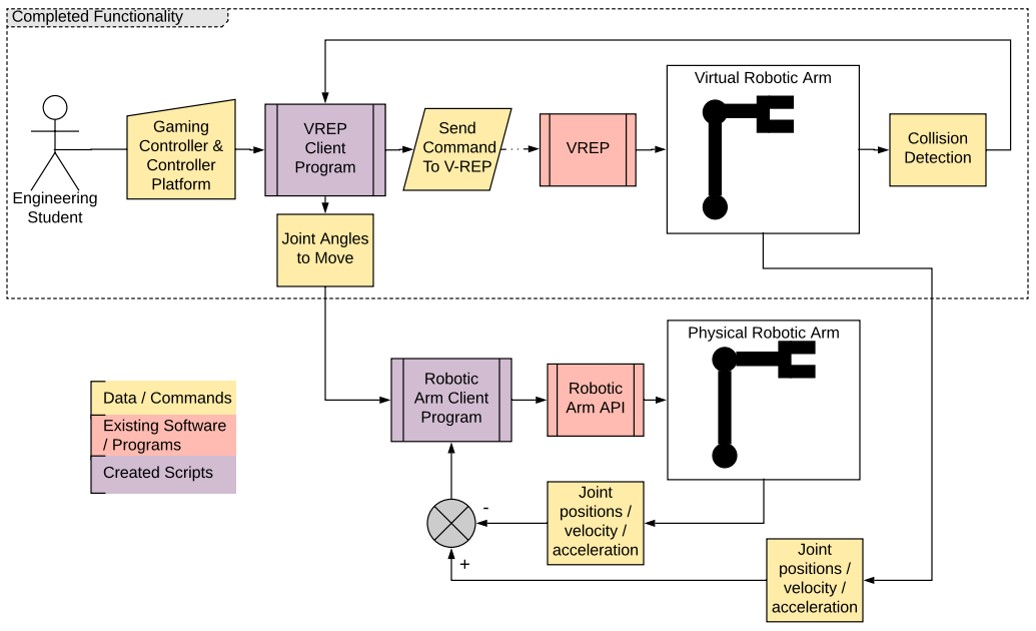
\includegraphics[width=1.12\linewidth]{Thesis_flow_chart.jpg}
\caption{Flow diagram describing the key features of this thesis}
\end{figure}
\end{center}


% leading introduction statement
From here, a variety of challenges will be pondered as mathematical formulas are derived to describe the motion of a 6 degree of freedom (DOF) arm, and a remote interface is created for allowing real-time movement within VREP.\\

%% default intro
%The introductory chapter describes the importance of the field and the
%scope and significance of your project.  It usually ends with an
%overview of the remainder of the thesis.%
%
%Notice that Arabic page numbering begins with Chapter 1.  Preceding
%pages (known as ``frontmatter'') have Roman numbering.  The
%\texttt{book} document class in \LaTeX\ follows this numbering
%convention by default (see Lamport~\cite{lamport}, p.\,80).
%%
%%\chapter{Literature review / prior art}
%
%You will need to review previous work in the field, which may include
%books and papers (``literature''), patents and commercial products
%(``prior art''), and earlier work in your Department.  This
%information is usually (but not always) collected in a single chapter,
%whose title should preferably be more specific and interesting than
%the one above.
\chapter{Programming Robots to Move}
%% Go through case studies of how robots have been programmed to move in the past
In order to move a robotic arm, two layers of control are required, the motor position control for each joint, and the system that depicts how much the joints need to change angle when moving from one arm configuration to another. Following are some case studies that present methods of controlling a robotic arm, where the maths behind them are left for the theory section of this report.

\section{MATLAB Toolboxes}
Matlab provides an extraordinary amount of support for calculating the important properties required for the control of a robotic manipulator. Below is a sample of some of the useful libraries available that were, and further could be, beneficial to creating an interface for controlling the virtual Kinova Jaco arm remotely.

\subsection{Robotics Toolbox}
%https://robotacademy.net.au/masterclass/inverse-kinematics-and-robot-motion/?lesson=301
Professor Peter Corke, the Director of the Australian Centre for Robotic Vision (ACRV), has designed a Matlab specific toolbox for computing the mechanics associated with robotic manipulators. Included is easy to use functions for creating robotic arms, and calculating parameters such as forward and inverse kinematics, trajectory generation and control systems for motor control. Within the Queensland University of Technology's Robot Academy is 'Master Classes' on using the toolbox through examples of simple manipulators and the theory behind the complex calculus being performed.\\

There are dozens of object files containing the parameters of robotic manipulators; including the 6 DOF puma560 and limited information on the 6DOF Kinova Jaco arm. The parameters within these files contain the link times of the arm, the Denavit-Hartenberg parameters (DH parameters - theory section of this report), and can contain inertial and angle properties for each link. These properties are helpful in computing the forward kinematics, inverse kinematics, and dynamic equation representing the motion and torques on the arm.

With this, the toolbox allows the viewing of the manipulator in desired angles, the movement of the arm between two desired end-effector positions, and the building of the control system controlling the torque at each motor given the current arm configuration. The latter of which is crucially important in providing accurate control of the arm, in ensuring the appropriate power is provided to all of the joint links as it moves over a given trajectory. Unfortunately, it is extremely difficult to compute, and for each degree of freedom contains 10 constants that need finding; mostly inertia terms which for each link depends on its orientation and position relative to the arm's base; thus relying on all link angles between the base and the link of interest. The mechanics of this is presented in the theory section of the report, but the Robotics Toolbox provides functions which compute the inertial, coriolis and gravitational torques acting on the arm. Professor Corke also provides a method of motor control for each link given the aforementioned parameters are known. The method uses the typical motor position control strategy of a Proportional Derivative Controller (details in the theory section) to compute the required motor torque from the error in angle position and velocity, however also includes a feed-forward component of the calculated disturbance torque due to the coupled dynamics between links. 

\begin{center}
\begin{figure}[htb]
  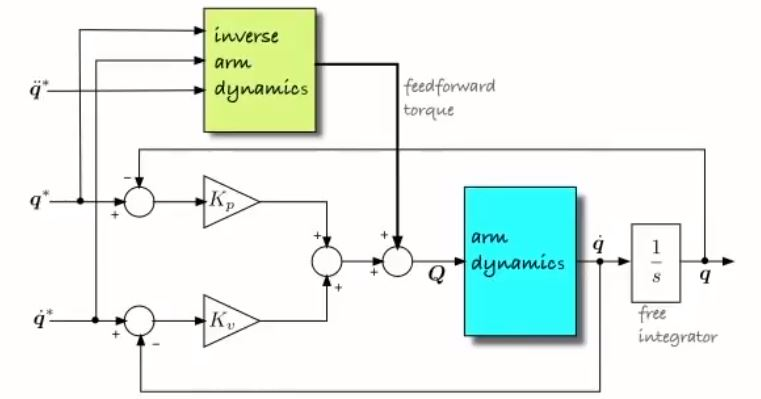
\includegraphics[width=\linewidth]{Correcting_for_disturbance_torque.jpg}
\caption{Motor Torque Control System}
\end{figure}
\end{center}

Thus the torque provided at each link can be expressed as:

$\tau = K_p (q^{*} - q) + K_v (\dot{q^{*}} - \dot{q}) + M(q) \ddot{q^{*}} + C_j (q, \dot{q}) \dot{q} + g_j (q)$

Where the change in angle required by each joint when moving the end-effector from one coordinate to another can be computed using the variation of the 'ikine' function for the given robotic arm; the forward kinematics can be computed similarly using the 'fkine' function.
%% this should be compared to how VREP controls the arm using PID in the theory section. Additionally, the advantage of calculating the dynamic equation for the arm for LQR

\subsection{Robotic Arm Models}
%https://au.mathworks.com/help/physmod/sm/ug/import-robot-arm-model.html
%https://au.mathworks.com/help/control/examples/multi-loop-pid-control-of-a-robot-arm.html?searchHighlight=robotic%20arm&s_tid=doc_srchtitle
Separate to the custom designed toolbox of Professor Corke, MATLAB has its own robot manipulator modelling sub-program and alternative methods of control. Simscape allows the creation of physical systems within MATLAB's simulation tool Simulink. An example of 6 DOF robotic arm is presented below; the base of the arm represents the origin, and the lines span out from this with rigid bodies followed by links. Each rigid body can be shaped within MATLAB or imported from a CAD model to produce a replica of the real robotic arm; where properties such as material and interia can be defined.

\begin{center}
\begin{figure}[htb]
  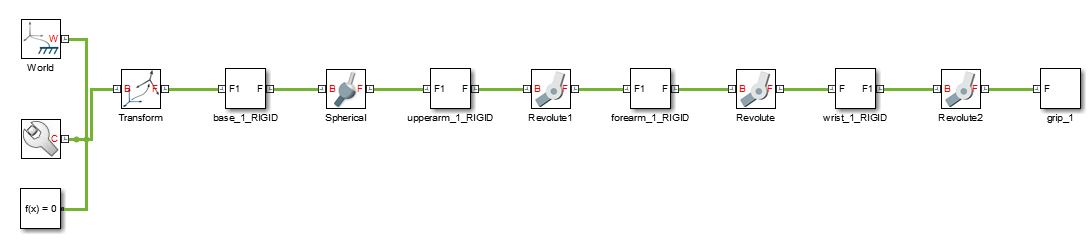
\includegraphics[width=\linewidth]{simscape_robotic_arm.jpg}
\caption{smrobot Simscape Model}
\end{figure}
\end{center}

Simulating the model shown above will provide a visualisation of the arms and any motion set on it by external forces or motor torques; not included in the above model.

\begin{center}
\begin{figure}[htb]
  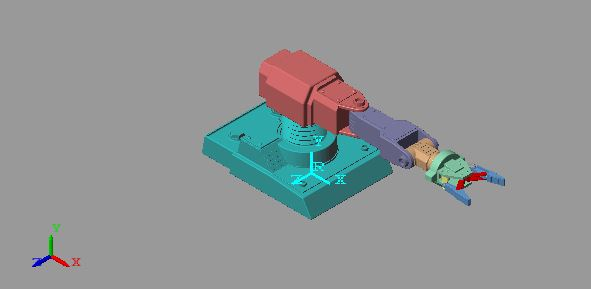
\includegraphics[width=\linewidth]{simscape_robotic_arm_model.jpg}
\caption{smrobot Simscape Model Visualisation}
\end{figure}
\end{center}

From here, it is a matter of controlling the robotic arm to move from one joint configuration to another. For a custom robotic arm, any of the strategies outlined in the theory section of this report can be used, however MATLAB provides another means which is described in the section below. In order to move the joints from one position to the next, a strategy similar to that shown in Figure 2.1 is required. In simulink, the layer of controlling the motor position can be formatted as follows:

\begin{center}
\begin{figure}[htb]
  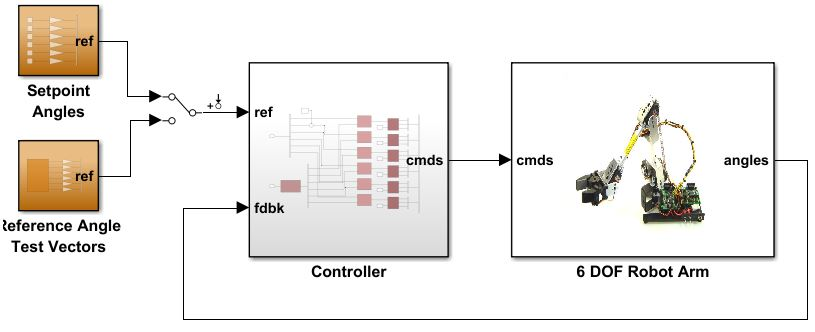
\includegraphics[width=\linewidth]{simulink_motor_control_loop.jpg}
\caption{Simulink Model of Motor Control Loop}
\end{figure}
\end{center}

Where nested within the controller is the tuned PID controllers for each motor which drives it to the desired position. This is similar to Peter Corke's method but without pre-emptive knowledge of the disturbance torque due to the arm's dynamic coupling.

\begin{center}
\begin{figure}[htb]
  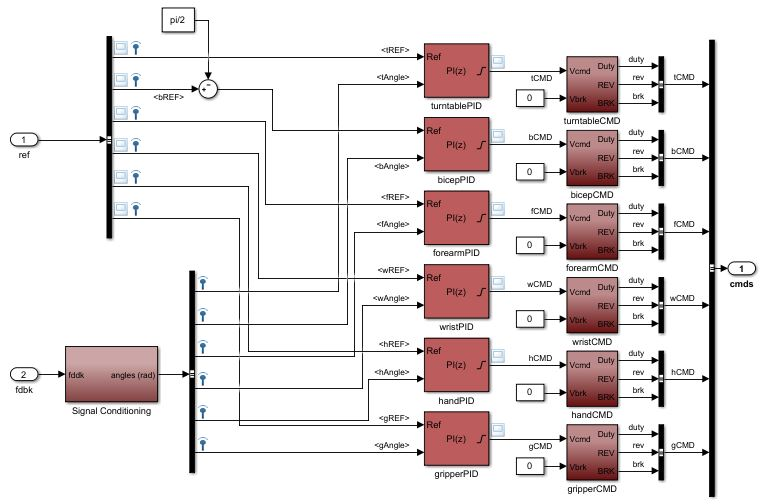
\includegraphics[width=\linewidth]{simulink_motor_control_PID.jpg}
\caption{Simulink Model of Motor Controllers}
\end{figure}
\end{center}

It will be seen that VREP operates in the same way, as it enables the importing of manipulator models and setting of each joint's controller coefficients. The figure above gives a good representation of the mechanics behind what the parameters are doing in terms of regulating each joint's error to a desired angle. A significant advantage of MATLAB is the auto-tuning functionality of the PID controllers for each joint, however a controller on it's own would not be as robust as that described in the Robotics Toolbox section.

\subsection{Adaptive Neuro-Fuzzy Inference System}
%https://au.mathworks.com/help/fuzzy/modeling-inverse-kinematics-in-a-robotic-arm.html?searchHighlight=robotic%20arm&s_tid=doc_srchtitle
An Adaptive Neuro-Fuzzy Inference System (ANFIS) network can be used to deduce the joint angles required for an arm's end-effector to reach a desired 3-D position. Calculating the required angles analytically for an arm of greater than 4 DOF can become challenging and result in infinitely many solutions. Like any neural network, with a sufficiently large dataset the internal weights will learn what angles will result in the desired end-effector position. Thus, in training an ANFIS to control each joint for a training dataset, it is able to interpolate angles to sufficient accuracy and move the joints to reach a desired end-effector position.

To train the network, input to output mapping data is required. Thus, given the forward kinematics for a robotic manipulator is known, a dataset of angles to end-effector position can be created over the space that it is desired for the end-effector to move. After the network gains its own understanding of the mapping, any point within the testing region can be given and the network return the required joint angles. In a MATLAB example, each joint is given its own network to be trained such that for each joint an angle will be provided given a desired position. Outside the range of training, the manipulator will not respond promisingly, and thus for a large control range, a sufficiently large dataset is required. Overall neural networks respond quickly to providing results once trained, however the training process can be time consuming.

\section{Programmed Robotic Arms}
%https://pdfs.semanticscholar.org/75f2/fa10a66e35bd6b5b5d695b31be51df78303e.pdf
Volume 58 of the 2012 International Journal of Computer Applications, titled Software Development for an Inverse Kinematics of Seven-Degrees of Freedon Newly Designed Articulated Inspection Robot, details on previous software development tools used to control robotic manipulators. It is detailed that the inverse kinematics can be solved using an Adaptive Neuro Fuzzy Network (ANFIS), a neural network trained to reduce error in end effector position, non-linear optimization methods, geometric approaches, and through the manipulation of the transformation matrices. In the ANFIS approach, it was noted that MATLAB was used, however C / C++ programming has been used to develop programs that compute the more mathematics based inverse kinematics methods. A program is proposed in this paper which uses Visual-Basic to allow the calculation of forward and inverse kinematics, and trajectory planning.\\



%http://scholarcommons.usf.edu/cgi/viewcontent.cgi?article=2791&context=etd
A thesis paper from the University of South Florida comments on the fact that programming in a low level language such as C is closer to the hardware level which reduces computation time in processing and communicating with external systems (sensors and motors). High-level languages, such as MATLAB, provide an user-friendly interface for solving complex maths operations, however lack capabilities found in C / C++ such has multi-threading and easy communication between concurrently running processes. It is explained that the complexity in configuring MATLAB to communicate with a separate C++ program lead to failure of the wheel-chair mounted robotic arm's program on multiple occasions. The software system in this paper refers to using a C++ program used to communicate with sensors and other hardware, whilst using MATLAB for the control algorithm computations, and simulation. Due to the aforementioned advantages of C++, a new C++ program, with an external library for matrix manipulation, was created to replace the MATLAB program. The concluding results being that the new software system reduced delays in the control of the robotic arm, leading to better stability and control.\\
The primary purpose of using MATLAB in this experiment was to simulate a virtual model of the robotic arm, and using the angles of this to control the physical robotic arm through the C++ platform. The complexity and delay produced by MATLAB lead to slow and unreliable control.\\



The Kinova Jaco arm's Software Development Kit (SDK) is written in C++, with the handling of communication and calculations stored in an human-unreadable dynamic link library. There is no documentation into how the SDK calculates the joint angles required for a desired gripper position, however there are usage examples in C++ of all the available functions; one of which is used to setting the gripper position and angle in cartesian coordinates. This SDK allows direct tuning of crucial arm parameters such as maximum applied torque, PID coefficients and velocity control. Predefined structures can be filled with this information and sent to the arm's FIFO buffer to interpret and act accordingly, making the control of the arm from the developer's perspective effortless.\\
Controlling the robotic arm in this way however, means the arm needs to be completely set-up in order to use the SDK. It may also be hard to understand how the parameters affect the movement of the arm; for example, the coordinate system isn't well defined and will take some trial and error to understand. This could be done with the help of the `get` functions, which can return torque, velocity and position values of the arms current configuration. To further understand how the settings can affect the arm, Kinova have supplied the `Development Center` with the SDK (which back-end C++ code is accessible, and can provide knowledge into how the arm can be controlled) what allows the user to move the arm, set trajectories, and review current parameters.\\



% I really don't know much about ROS... RVIZ?
%http://wiki.ros.org/ROS/Introduction
%https://github.com/Kinovarobotics/kinova-ros
The Robot Operating System (ROS) is a modular collection of commonly used software in low-level device control, hardware abstraction and functionality seen in robotics. ROS can be used in Python, C++ and Lisp programming languages to build a framework around robotic software kits that directly control a robotic actuator. Thus, it has already been used as a cover of the Kinova SDK for the Jaco arm. Further, simulation platforms such as Gazebo and MoveIt can be controlled using ROS, with the software for controlling a Jaco arm in Gazebo being available. Together, ROS can be used to control a virtual model of the Jaco arm in Gazebo, as well as the physical arm through the Kinova SDK. Control of robotic manipulators in VREP is also available using ROS through the VREP remote API.\\
%https://pdfs.semanticscholar.org/2600/e3b018b5fa77035dab558f783919c9d46d35.pdf
ROS offers a package called Rvis, which provides a method of interacting with imported models in 3D. Similar to a robotics simulation package, Rvis can provide information about the centre of mass of objects, collisions, and joints of robotic manipulators and objects in a scene. It however lacks the real-world modelling that comes with simulation programs such as V-REP or Gazebo (running a physics engine). Thus, it is typically used as a wrapper for these programs, such that the user can retrieve key information about objects in a scene whilst simulating properties such as gravity and friction.


%https://robotacademy.net.au/lesson/inverting-the-jacobian-matrix-2/
In Professor Peter Corke's Robot Academy series, he goes through an intuitive explanation for programming robotic arms using the arm's Jacobian matrix (referenced in Theory). As the Jacobian is a function of joint angles, it only provides a truthful reflection of the small change in angles required for a small change in end effector position, local to the current arm configuration. Thus, the Jacobian matrix can give a solution for small angle changes, but after the arm moves to this new position, it must be recalculated. This can be done in programming using discrete time steps as outlined in the figure below. Unfortunately, as this is an approximation technique, if any of the spacial or time parameters are too large, the result will no longer hold, and thus it should be used with caution.

\begin{center}
\begin{figure}[htb]
  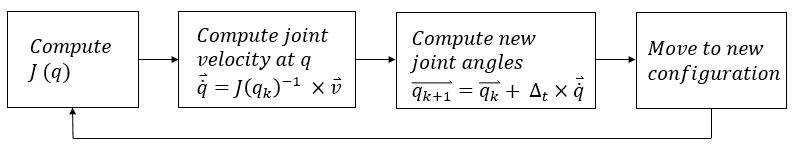
\includegraphics[width=\linewidth]{jacobian_programming.jpg}
\caption{Flow Diagram of using Jacobian in Programming}
\end{figure}
\end{center}

A similar technique that can reduce the error between the end effector's position and a small change in position is the PID controller. With the appropriate weightings for each joint, the joints can be moved to reduce the error in end effector position. Note that there is no control of the joint-space in this case, and could lead to undesired joint configurations. This gives the Jacobian an advantage, as it is non-invertible at a joint singularity; when the arm looses a degree of freedom.


\section{Simulation Platforms and Physics Engines}
%https://www.smashingrobotics.com/most-advanced-and-used-robotics-simulation-software/
There are numerous platforms available for simulating the dynamics and interactions of robot's with a scene. V-REP is particularly useful for this thesis due to its ability to remotely control the simulation and the objects within, whilst providing a realistic environment for said interactions. Other popular robotic platforms have similar functionality, but may come at a cost, include Webots, Robot Studio, ARGoS, labVIEW, Visual Components, Virtual Robotics Toolkit, Gazebo, Actin Simulation and Workspace. Although the objective of these platforms is to simulate a robotic manipulator in a scene, they are customized in the robots that can be simulated, the physics engine they use to simulate the dynamics, and the requirements by the users using the product. A good example of this is the Robot Virtual Worlds platform, which has comprehensive capabilities in simulating and programming LEGO robotics. On the contary, Workspace is used for simulating industrial production lines with multiple robotic manipulators acting together; and is used by large companies such as ABB and Mitsubishi. The scope of this thesis focuses on the use of free simulators that provide realistic and programmable simulations for educational use. Thus, simulation platforms such as Webots, Gazebo and V-REP are of particular interest as they equally provide the required features to meet the objectives. 

%https://arxiv.org/pdf/1402.7050.pdf
An online survey was conducted by researchers Serena Ivaldi, Vincent Padois and Franceso Nori to determine which simulation platform and dynamics solver was most preferred. The survey was completed by 119 participants with 62\% possessing a PhD, and of the remaining, 32\% had a university level degree. It was found that 39\% of the participants hadn't heard of V-REP, compared to 27\% and 15\% for Webots and Gazebo respectively. However, it was found that V-REP was the best rated for usability, documentation and set-up guides, whereas Gazebo was the most used. From the findings, it was noted that V-REP was the most likely for applicants to try, and keep using, compared to Webots and Gazebo.

%http://www.dca.fee.unicamp.br/~gudwin/courses/IA889/2014/IA889-02.pdf
A full comparison between Gazebo and V-REP was conducted by Lucas Noguira from the Universidade de Campinas. This article goes through implementing features common to both platforms and the process required for setting them up to do a given task; i.e. connect a sensor to a robot and read it through ROS. It was found that V-REP offered a much better interface for adding components, and used less computation time when compared. 

\subsection{V-REP}
% Introduce V-REP
The robotics simulation platform used in this thesis is the Virtual Robotics Experimental Platform (V-REP) by Coppelia Robotics. V-REP offers a means of realistically simulating mobile robotics and actuators with an easy to use interface. In a simulation, V-REP continuously reads an internal `main` Lua script, that may read other scripts describing properties associated with robotics in the scene, which are customisable by the user. On the side pane is a large list of available robots that can be imported, and once they are, a script customised by Coppelia is loaded to the list of running scripts; i.e. in the case of the Jaco arm, a script is imported that moves the arm around in the scene to a pre-configured trajectory. The simulation process is described by the figure below, where it can be seen that the main flow of code goes between actuation, reaction, sensing and control, with monitoring collisions being the main priority at each stage.

\begin{center}
\begin{figure}[htb]
  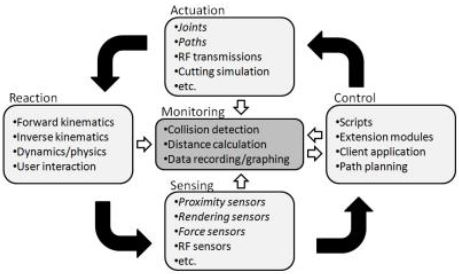
\includegraphics[width=\linewidth]{vrep_simulation_diagram.jpg}
\caption{Flow Diagram of the V-REP Simulation}
\end{figure}
\end{center}

\subsubsection{Communication}
%Introduce a means of communicating with V-REP
%http://www.coppeliarobotics.com/helpFiles/en/writingCode.htm#sixMethods
Fortunately, the parameters within these scripts and objects within the scene can be controlled using the remote API, which is available for C/C++, Python, Java, Matlab, Octava, Lua and Urbi. The documentation for the remote API contains extensive descriptions of over 100 functions, where the usage is available for all supported languages. Additionally to the remote API and internal Lua scripts, there are 4 other methods of controlling a scene in V-REP. The most obvious is plugins, which can provide custom Lua commands for interacting with the internal Lua scripts, it is effectively an external library of functions. Similarly, ROS can provide a wrapper of V-REP, enabling control from any ROS supported coding language, and further can enable the control of an external robot through a ROS node, using the information from V-REP; which is the aim of this thesis to a large extent. ROS. There is no limitations to utilizing V-REP's capabilities between using a remote API client and a ROS node, as seen in the connection methods table on the V-REP website; both will contain lag due to communication over the internet through a socket connection. Other methods of controlling V-REP include through the use of an add-on, or a BlueZero node.

%Introduce the methods of communication with V-REP remote API
Communication using the remote API is through a socket connection between the client API and VREP. To enable connection, V-REP needs to be configured to allow external connections through a specified port; there is no restriction to the number of open ports, however it does induce simulation lag. As scripts are associated with objects within the scene, this configuration is typically set in a threaded child script of an invisible dummy object in the V-REP scene; an example of this can be seen below. 

\begin{center}
\begin{figure}[htb]
  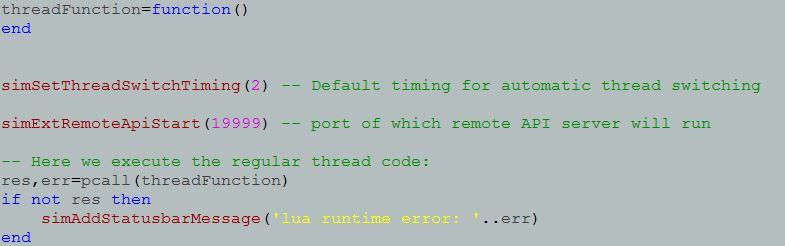
\includegraphics[width=\linewidth]{vrep_port_listen.jpg}
\caption{Sample Lua Code for Connecting V-REP to a port}
\end{figure}
\end{center}
%http://www.coppeliarobotics.com/helpFiles/en/remoteApiFunctions.htm
On the client side, connecting to V-REP waits for a given length of time for a client identification number. Once this number is obtained, the number is used for all communication thereafter in a manner noted by Coppelia for the language chosen. As an example, the functions could return parameters such as joint angles, velocity and sensor outputs, alternatively the functions could also be used to set or change these parameters.
% need to discuss at some stage that communication isn't guaranteed between different networks, i.e. home verse uni

Communication between the client program and V-REP is undertaken in four different modes; blocking function calls, non-blocking function calls, data streaming and synchronous operation.

\begin{center}
\begin{table}[htb]


    \begin{tabular}{ | l | p{10cm} |}
    \hline
    Operation Mode & Summary \\ \hline
     Blocking & When a command is sent in blocking mode, the client will wait until the V-REP API response before moving to the next line of code.\\ \hline
    Non-blocking & When data needs to be updated in the client program, that isn't required straight away. The client can make a call for the data to be copied to a particular address and move on to the next line. The API will respond in due time.  \\ \hline
    Data Streaming & When the same data is constantly required from V-REP, the data-streaming method allows a way for V-REP to send updates of a particular value without calling for it each time. For instance, joint angles of a robotic arm may be required by the client program with large frequency, and could be updated without making direct calls and waiting for a response each time once a data-streaming call is given. This is a continuous mode, and the client will be stuck receiving data. \\
    \hline
    Synchronous & When it is desired to have the simulation and client program run concurrently in time, such that the simulation advances with the client. Synchronous mode allows the client to control the advancement of the simulation.\\
    \hline
    \end{tabular}
    \caption{V-REP remote API operation modes}
\end{table}
\end{center}

To be able to interact with a particular object in V-REP, one must refer to it in function calls using its `object handle`. The object handle is a unique number given to every object in a scene, typically in order of when the object was added to the scene, known by its appearance in the scene hierarchy; a list containing all of the objects in the scene, starting with objects like the default camera, floor, lights, XYZ coordinate frame, and then any objects that were placed in the scene after. Once an object has been deleted from the middle of the hierarchy, the other objects retain their object handle; thus once an item is added its object handle won't change. When calling a missing object in a scene, NULL will be returned.

\subsubsection{V-REP Features}

Models can be imported into V-REP as a mesh (.stl) from any 3D modelling software (such as AutoDesk). The models can either be static objects to be placed in the scene, or make up parts of a robotic manipulator. When importing models, it is important to consider the amount of triangles used to create the component, when this is too large (more than 20,000), manipulating the object in V-REP will come with noticeable lag. When building a robotic arm from a CAD drawing, the entire model can be imported, and then subdivided to form an interaction `group` of meshes. When the Denavit-Hartenberg parameters of the arm are known, these can be used to form the relationship between the joints. The interactions between parts can be made by adding translational and/or rotational relationships, with parameters such as maximum angle and starting position specified. All of the objects in the scene can be modified out of simulation to be dynamic or static (be influenced by external forces), and responsive or non-responsive (have a reaction when a collision with the object occurs). It should be noted that the object doesn't need to be part of a robot, but can be an object in the scene either as a feature or an interactable object.\\


On start-up, V-REP comes with 21 pre-assembled non-mobile robotic manipulators (arms), including the Kinova Jaco and Mico arms. Other V-REP supported models can be loaded into a scene, given the appropriate .ttm format. The model browser also includes a selection of pre-made models, such as arm grippers, sensors, furniture, household appliances, people, vehicles and mobile robots. Using the model browser alone, it is possible to replicate a room or scene that a real robot would interact with. The robots can also be placed on any surface in the scene, and be provided a given trajectory or motion path for interacting with objects.\\


Collision detection is an important feature required for this thesis, as the objective is to detect collisions within the scene. V-REP has a collision detection feature, which will register collisions between collidable entity-pairs. Thus, objects that may collide within a scene need to be set prior to simulation; a robotic arm can be set to 'Enable all collision detections', which will flag when the robotic arm collides with any object. From a remote API client's prospective, this isn't yet helpful as V-REP will not flag a collision to the client automatically. Instead, the client program will need to ask for the execution of a custom Lua function within V-REP, which will use the simCheckCollision function to check for collisions within the scene, and then stream the response back to the client. Thus, this could be used in a data-streaming method, where the client is continuously checking for data from V-REP being send from the custom function. Alternatively, the remote API contains a simxReadCollision function which can be called given an object's collision handle (i.e. a link of a robotic arm pre-registered to potentially collide), where the response will indicate a collision or lack there of.\\


%% need to go into the inverse - forwards kinematics... Still not sure how they solve for these given any model can be created in V-REP...
The most useful feature of V-REP's for this thesis is the kinematics solver, where the arm can be set to either forward kinematics or inverse kinematics mode. By default, one is able to give joints desired positions, and the PID controller representing the motor dynamics actuates the joint to produce a realistic resulting position at that of which is desired; unless the motor actuation saturates, resulting in steady-state error from the goal position. From the V-REP client, one is able to send desired position, velocity and actuation force to the joints of a robotic manipulator at any given moment. Conversely, when the position of a joint in space is desired, the calculation of the angles to produce this goal position is required. V-REP is able to solve this inverse kinematics problem, given a desired position, the links requiring moving and the joint position to be moved are known; and the desired position is in reach of the arm, i.e. the solution is solvable.\\
To set a robotic arm to inverse kinematics mode such that the end-effector reaches a goal position, a dummy object representing the `Target` for the gripper must be added. It may be desirable to also create a `Tip` dummy object that moves with the gripper, at a position defined as the tip by the forward kinematics transformation for the arm. This tip object is required to be nested under the gripper parent on the scene hierarchy, such that it moves with the gripper, however its world coordinate can be set to that of the forward kinematics solution at any moment, and this offset to its parent will be maintained.\\
The `Scene Object Properties` for the dummy objects depict the kinematics mode and the links to other objects in the scene. In this window, the objects would be required to be set to non-collidable, non-measurable and non-detectable, so they are merely position orientated objects. Further, once the inverse kinematics link between the objects is made, V-REP offers the user to select between two inverse kinematics solutions in the `Calculation Module Properties` window. These are the pseudo-inverse and damped least squares methods which are discussed in the theory section. Depending on the chosen method, the damping and number of loop iterations on evaluating an accurate solution can be set.\\

\subsection{Alternative Simulation Tools}

\subsubsection{Webots}
%http://journals.sagepub.com/doi/pdf/10.5772/5618
Webots is a robotics platform that allows the simulation of popular robot models, that can be interacted with using external software scripts, of which can be then programmed onto real robots; given they are compatible. Similar to V-REP, one can communicate with the simulation using TCP/IP from a program written in C/C++, MATLAB, Python or Java. The simulation also utilises Open Dynamics Engine (ODE) to give a realistic representation of physical interactions between objects. Motors and sensors can be placed in the scene or within robots, and tuned to mimic their real-time capabilities; maximum torque, PI control of servos, and sampling of sensors to name a few parameters that can be varied. There is little information on the comparison between this platform and V-REP, but from the information found on Webots and in the survey outlined above, it appears to have equivalent functionality, if not less, as it relies only on one physics engine whereas V-REP offers four.
Webots could be used for this thesis, as it provides a means of real-time (or even speed-up) interaction with a scene and the objects within. The use of ODE is no downfall, as outlined in the ODE section, it provides a realistic rendering of collisions within a scene.

\subsubsection{Gazebo}
%http://lenkaspace.net/blog/show/120
Gazebo offers a very similar platform to V-REP, where a model can be placed in a scene and have the simulation controlled by a remote API. As an open source platform, full integration with ROS has been created, where the internal parameters of a simulation can be controlled with ROS. It is offered on any OS with a command line interface to help control simulations. Simulations are saved to an .xml script, which can be edited, and rerun; a feature V-REP lacks with it's .ttt saving format. A thorough comparison was made between Gazebo, V-REP and ARGoS, which demonstrates that they both contain the key features required for this thesis. It can be seen however, that V-REP has more positive features when compared to the other too. Gazebo on start-up is build with ODE, however can be built from source with any physics engine.

\subsubsection{Bullet Physics Library}

\subsubsection{Open Dynamics Engine}

\subsubsection{Vortex Dynamics}

\subsubsection{Newton Dynamics}



\chapter{Theory}
In order to ensure the client program can function responsively, control the robotic arm in real-time and not over-use the computer's CPU, a variety of theory had to be researched before commencing the project. In particular, the theory examined covered three main areas; the mathematics associated with the dynamics of non-linear systems, control theory, and software development. As this is a Mechatronics thesis, key theory of these topics will be explained for the interest of the reader, in-case their expertise are not refreshed in these areas.

\section{Child Processes and Multi-Threading}
Processes have their own memory-space and are are completely separate to one another. They are able to interact with their virtual memory and create threads to undertake separate tasks, such as getting inputs from a user, handling the graphical interface, writing external hardware. A process is effectively the application or program as a whole, and threads are the internal functionality that coordinate information that make up the program. Threads have the appearance to be working in parallel, but synchronously; for instance, one thread may be checking for a particular sensor reading, and once this has been received it can signal to another thread, that is waiting for the signal, to conduct calculations or react in particular manner. Threads have their own stack and priority, and so variables local to one thread doesn't affect another's, however as noted, they are able to signal each other, as well as share the process's data (i.e. global variables). This is a vital difference between processes and threads, processes cannot effect each other's memory, they have allocated space and interact with Kernel on how much memory it can use, but it cannot access another process's variables. All application processes have the same priority also, whereas threads can have a variety on different priorities depending on CPU time and importance to the overall functionality. As a rule of thumb, threads that make important calculations and run quickly have high priority, whereas slower threads doing large tasks can have a lower priority, because compared to their overall CPU time blocking for a fast thread won't greatly effect the runtime.\\


Typically, when developing an application in a coding language such as Python, MATLAB and C, the flow of code is singular as there is one process and one thread. The main thread in a program can create other threads, which are given a unique thread identification. In the same way, a process can spawn another process with a unique process identification number, however obtains a parent process identification number. In this way, the parent process can monitor the status of the child process, and send signals, similar to threads. \\
%https://linux.die.net/man/2/fork
In Linux, the child process is created by duplicating the parent, and giving the new process it's own resources such as memory-space and timers. The processes can communicate through reading and writing to files in memory and signalling that messages are ready; this is called piping, where an output from one process serves as in input to another. When using the Windows API however, the set-up is slightly different, in that everything is a `Window`, and Windows send messages to other Windows. The intuition behind this is that a Window can be interacted with by the user at any time, with key strokes or mouse clicks, and from operating system events. Thus, when a Window is created, it is set-up to receive signals through a queue that will hold messages, so it is ready when these different events occur, enabling it to react accordingly. Between operating systems, the overall outcome and the way processes interact is in essence the same, however when programming these differences become noticeable as each has their own checks, structure and signalling.\\
%https://msdn.microsoft.com/en-us/library/windows/desktop/ff381405(v=vs.85).aspx

The CPU is a shared resource between processes, where the CPU usage for a given process is calculated as a percentage of the amount of clock cycles dedicated to running a particular task/thread. As aforementioned, threads can be allocated priorities, and thus if the threads of a process are constantly requiring run-time, say being stuck in an infinite loop, the CPU will be held servicing the one process given no task of higher priority is scheduled, thus consuming 100\% of the CPU usage. On a program level, if tasks are of equal priority and in no way get suspended, the CPU will schedule the run-time of the tasks equally between them.\\
To avoid having a program use up all of the CPU's available usage, by taking the CPU whenever it becomes available, threads are suspended whilst they wait for information. Suspended threads can be resumed by events such as receiving a signal from another thread, or a given amount of time has passed. It is in this way that the CPU is able to run multiple programs concurrently, threads will block until they are required to be serviced, and until then the processor can run other tasks. An example of this is the USB ports in a computer, the processor will run programs, and occasionally stop and check the hardware states of the computer, before re-storing the memory of a suspended program and resuming. When a USB is connected, the hardware task will signal that one of the ports is in use, and begin a chain of events, taking priority over the program that was running. \\
Threads can be suspended in programs typically by a function called sleep, which is given a specific amount of time to sleep for. The function for resuming suspended tasks will also exist, which typically requires a handle to the thread in memory.\\


\section{Regulators}
The fundamental definition of a linear system is a system that when given a harmonic input, produces a harmonic output. Due to the frequency characteristics of the system, the output may be scaled and phase shifted, however the harmonic remains. In this sense, the input shapes the output. Regulators are a class of control scheme that use this property to shape a desired output given a reference input, with the use of feedback and a compensator.
\\
\begin{center}
\begin{figure}[htb]
  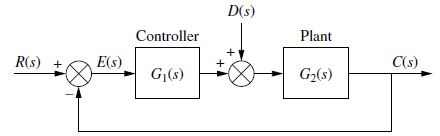
\includegraphics[width=\linewidth]{feedback_control.jpg}
\caption{Feedback Control System with Disturbance}
\end{figure}
\end{center}
%% Reference from p356 of Nise Control Systems textbook
 Presented in the figure above is a simple control system which contains a plant that takes input from a controller, which is driven by an input defined by the reference input R(s) and output C(s); although the laplace notation is used in this figure, R and C could the state vectors of the system. Ignoring the disturbance at this the system in this thesis is virtual, it is known that the gain for this type of system is defined as;

$\frac{C(s)}{R(s)} = \frac{G_1(s) G_2(2)}{ 1 + G_1(s) G_2 (s)}$

and the error is;

$E(s) = \frac{R(s)}{1 + G_1(s) G_2(s)}$

where controllers $G_1(s)$ are designed to minimize $E(s)$,such that the steady-state error is zero;

$e(\infty) = \lim_{s\to0} s * E(s) = 0$

A typical example of a controller has already been mentioned in this paper, and that is the PI (proportional gain plus integral action controller) which was proposed for regulating the servo positions inside a robotic manipulator's joints to a desired joint position. In that circumstance, the controller is defined by the function;

$ G_1 (s) = \frac{K_P s + K_I}{s}$
where $K_P$ and $K_I$ are the proportional and integral gains respectively. In this case, the controller takes in error in servo angle and outputs a voltage that goes to the motor to produce the desired reference on the output. The reason a PI controller is used in this case is due to the integral action's ability to reduce steady state error. This is easily analogous when considering a mechanical system being moved to a desired position. The proportional gain multiplies by the current error to produce a force that moves the system, however there is no judging whether this force is enough to overcome the opposing forces in the system, and may result in an equilibrium position less than that of which is desired. The integral of the error can thus be used, as the error accumulates and gets multiplied by $K_I$, the force grows to overcome the disturbances until the desired location is reached. This can be seen when considering the steady-state error formula with the referenced controller and a mechanical plant with inertial and linear components (thus, at minimum be defined by $[M]s^2 + [K]$);

$ \lim_{s\to0} s * E(s) = s * \frac{R(s)}{1 + \frac{K_P s + K_I}{s} G_2(s)}$

$ \rightarrow e(\infty) = \lim_{s\to0} s   \frac{s   R(s)}{s + (K_P s + K_I) G_2(s)} = \lim_{s\to0} \frac{0}{K_I G_2 (0)} = 0$

Thus integral gain eliminates steady-state error given sufficient time, hence its use as a regulator in servo motors. The use of controllers cannot be mistreated however, as it may have been realised in the mechanical example above, the gains will change the dynamics of the system. Thus, when using controller's it is required that they are tuned to give the desired damping, rise-time and settling time of which is required for the system. In general, the addition of $K_I$ increases overshoot and settling time, which can be counter-acted by the inclusion of a velocity term $K_D$, which for a second order system will decrease overshoot, but incorporate delay into the system. Another negative with using a derivative controller as a regulator in the feed-forward path is that it can lead to over-saturation of the actuator when the reference input is changed between two consequent time samples (step change), producing a 'infinite' gain being multiplied through the plant. The proportional gain is similar to $K_I$, in that if sufficiently large can cause overshoot of the desired position, however, will always result in steady-state error.

This thesis looks into the use of controllers to correct for the error between the desired end-effector position, and the actual. It is proposed that regulating the coordinate space of the end-effector can be achieved by varying the joint angles of the arm with a controller based off the joints' sensitivity in moving the end-effector in a given direction. The premise behind the methodology chosen is backed by the theory presented in this section.\\


%http://www4.cs.umanitoba.ca/~jacky/Robotics/Papers/spong_kinematics.pdf
\section{Forward Kinematics}
As previously mentioned, the forward kinematics of a robotic chain is mathematics that defines the relationship between known joint angles and the end-effect position, such that
$\vec{P} = f( \vec{q} )$ \\
where $\vec{P}$ is the position vector of the end-effector relative to the base of the arm and $\vec{q}$ is a vector of joint angles $\theta_i$ or prismatic joint displacements $d_i$.

This function, $f(\vec{q})$, is found by the translational components of the transformation matrix, $T$, that describes the sequence of twists, rotations and displacements between end-effector position and base of the chain. $T$ can be found by multiplying the transformation between the base link and the next due to $q_1$, by the transformation between the next link and that after due to $q_2$, and so on until the end of the arm, denoted as link number $n$, such that;

$T = A_{0}^i = A_{0}^{1} A_{1}^{2} ... A_{n-1}^n$

The homogenous transformation between two links, $A_{i}^{i+1}$, is created using the product of the rotational transformation about the (rotation axis) z-axis, the translation transform along the z-axis a displacement $d_i$ (the offset in the z-axis from one link to another), the translation transform along the x-axis a displacement $a_i$, and finally the rotational transformation describing the rotation from one x-axis of first joint to the same of the next by an angle denoted $\alpha_i$. These terms are the Denavit-Hartenberg Parameters for the robotic chain, and can be further understood in the figure below provided by Mark W. Spong's Robot Modeling and Control textbook;

\begin{center}
\begin{figure}[htb]
  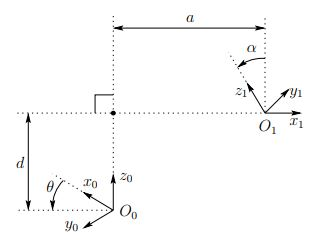
\includegraphics[width=0.5\linewidth]{DH_Parameters_figure.jpg}
\caption{Physical representation of D-H Parameters between two links}
\end{figure}
\end{center}

Where it can be seen that two criteria must be met for the transformation to exist, $z_0$ intersects $x_1$, and axis $x_1$ is perpendicular to axis $z_0$.

\vspace{\baselineskip}
Thus, $A_{i}^{i+1}$ is defined as;

\vspace{\baselineskip}
$A_{i}^{i+i} = Rot_{z,\theta_i} Trans_{z, d_i}, Trans_{x, a_i} Rot_{x, \alpha_i}$

where
\vspace{\baselineskip}
$Rot_{z,\theta_i} =$
$
 \left(\begin{array}{cccc} c_{\theta_i} & -s_{\theta_i} & 0 & 0\\ s_{\theta_i} & c_{\theta_i} & 0 & 0\\ 0 & 0 & 1 & 0\\ 0 & 0 & 0 & 1 \end{array}\right)
$
, 
$Trans_{z, d_i} =$
$
 \left(\begin{array}{cccc} 1 & 0 & 0 & 0\\ 0 & 1 & 0 & 0\\ 0 & 0 & 1 & d_i\\ 0 & 0 & 0 & 1 \end{array}\right)
$

\vspace{\baselineskip}

$Trans_{x, a_i} =$
$
 \left(\begin{array}{cccc} 1 & 0 & 0 & a_i\\ 0 & 1 & 0 & 0\\ 0 & 0 & 1 & 0\\ 0 & 0 & 0 & 1 \end{array}\right)
$
, 
$Rot_{x, \alpha_i} =$
$
 \left(\begin{array}{cccc} 1 & 0 & 0 & 0\\ 0 & c_{\alpha_i} & -s_{\alpha_i} & 0\\ 0 & s_{\alpha_i} & c_{\alpha_i} & 0\\ 0 & 0 & 0 & 1 \end{array}\right)
$
\vspace{\baselineskip}
Thus, the transformation between joints can be described as;
\vspace{\baselineskip}
$A_{i}^{i+1} = $
$ \left(\begin{array}{cccc} c_{\theta_i} & -s{\theta_i} c_{\alpha_i} & s_{\theta_i} s_{\alpha_i} & a_i c_{\theta_i}\\ s_{\theta_i} & c_{\theta_i}c_{\alpha_i} & -c{\theta_i}s{\alpha_i} & a_i s_{\theta_i}\\ 0 & s_{\alpha_i} & c_{\alpha_i} & d_i\\ 0 & 0 & 0 & 1 \end{array}\right)
$
\vspace{\baselineskip}
It can be seen that the homogenous transformation $A_{i}^{i+1}$ contains the 3 dimensional rotation transformation matrix from $i$ to $i+1$, and the column vector representing the translation transformation;
\vspace{\baselineskip}
$A_{i}^{i+1} = $
$ \left(\begin{array}{cccc} & Rot_{i}^{i+1} & & Trans_{i}^{i+1}  \\ 0 & 0 & 0 & 1 \end{array}\right)
$
\vspace{\baselineskip}
Thus, as $T = A_{0}^{1} A_{1}^{2} ... A_{n-1}^n$, $T$ will too have this form. In addition to this, the end-effector position, for arbitrary joint angles $\vec{q}$, can be found by extracting the translational column vector, such that;
\vspace{\baselineskip}
$\vec{P} = f( \vec{q} ) = Trans_{0}^{n} (\vec{q})$

\section{Inverse Kinematics}
The inverse kinematics of a robotic manipulator is the mathematics that defines the angles of the robotic given the position of the end-effector relative to the base of the arm. Using the formula from the previous section, the inverse kinematics can be written as;

$\vec{q} = f^{-1}( \vec{P} )$

Given the derivation from the last section, this computation isn't simple to compute, as the angle vector $\vec{q}$ can contain any number of joint angles, whereas the position vector of the end effector $\vec{P}$ is defined in ${\rm I\!R}^3$. For a 6 joint arm, this gives 6 unknowns and three equations.\\

There are numerous methods that present inverse kinematics solutions to any serial chain of joints; even when there is no known closed form solution. A paper by Gregory Z. Grudic, the University of British Columbia, called Iterative Inverse Kinematics with Manipulator Configuration Control and Proof of Convergence, lists many of the different methods in some detail, including the Tsai and Morgan's solution for a 6 revolute joint arm. A summary of popular solutions is provided in the appendix\\

In this thesis, the most common approaches are used to determine the joint angles required to move the Jaco arm's end effector. %Further methods are briefly meantioned and referenced in the inverse kinematics appendix.

\subsection{By Matrix Manipulation Approach}
As previously stated, the transformation that describes the end-effector relative to the base for a set of joint angles can be represented by T such that;
 $T = A_{0}^{1} A_{1}^{2} ... A_{n-1}^n$	eq1
 
From this equation, for a 6 joint arm, it can be determined that;
 
$(A_{0}^{1})^{-1} T = A_{1}^{2} A_{2}^{3} A_{3}^{4} A_{4}^{5} A_{6}^{6}$ eq2

In the Introduction to Robotics: Analysis, Systems, Applications textbook by Saeed B. Niku, it was proposed that mathematical relationships between joints can be found by multiplying both sides of the transformation equation described in eq1, by the inverse transformation between two joints, as seen in eq2. In doing this, it is known that the left hand side must equal the right hand side, however some entries between the left and right may not appear the same, despite being equivalent. From this fact, two entries can be equated together to write trigonometric relationships between joints. It was found that this property is most easily seen where angled twists appear between joints. By iteratively multiplying through by the inverse of a transformation matrix between two joints and inspecting the right and left side's elements, the equations for each joint angle was determined. 

\subsection{Analytical Approach}

A popular approach to solving the inverse kinematics of simple serial chains is by analytically solving the relationship between joints, from the base to the end-effector. This is easiest seen through example, provided by Lung-Wen Tsai's Robot Analysis textbook.

\begin{center}
\begin{figure}[htb]
  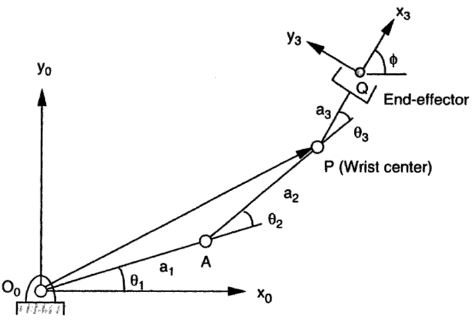
\includegraphics[width=0.8\linewidth]{Tsai_3rr.jpg}
\caption{Revolute Joint Arm}
\end{figure}
\end{center}

It can be seen in the figure above, that the end-effector is described by the coordinate vector $\vec{Q}$, with a joint 3 being represented in space by vector $\vec{P}$. It can also be seen that lengths $a_1$ and $a_2$ form a triangle with vector $\vec{P}$, dependent on the varying angles of $\theta_1$ and $\theta_2$. In addition to this, it can be seen that the four equations can be derived between the points;

$p_x = a_1 c\theta_1 + a_2 c \theta_{12}$\\
$p_y = a_1 s\theta_1 + a_2 s \theta_{12}$\\
$p_x = q_x - a_3 c\sigma$\\
$p_y = q_y - a_3 s\sigma$\\

where $\sigma = \theta_1 + \theta_2 + \theta_3$

From the cosine rule, the triangle can be defined by;

$p_x^2 + p_y^2 = a_1^2 + a_2^2 - 2 a_1 a_2 c \theta_2$

which can be rearranged for $\theta_2$ in terms of point P and the arm lengths such that;

$\theta_2 = cos^{-1} ( \frac{p_x^2 + p_y^2 - a_1^2 - a_2^2 }{2 a_1 a_2} )$
which will have two solutions depending on the evaluation of the fraction within the inverse cosine, and the arm is fully stretched when this equates to 1.

The equations describing $p_x, p_y$ in terms of $\theta_1, \theta_2$ above can be rearranged for $cos(\theta_1), sin(\theta_1)$ such that;

$c \theta_1 = \frac{p_x (a_1 + a_2 c \theta_2 ) + p_y a_2 s \theta_2}{a_1^2 + a_2^2 + 2 a_1 a_2 c \theta_2}$

$s \theta_1 = \frac{p_y (a_1 + a_2 c \theta_2 ) - p_x a_2 s \theta_2}{a_1^2 + a_2^2 + 2 a_1 a_2 c \theta_2}$

and $\theta_1$ can be computed by;

$\theta_1 = Atan2(s\theta_1, c\theta_1)$

Using the desired end-effector position Q, the third angle can thus be solved from its relationship to point P, described above. This method can be repeated working up the joints, were the position of each link can give the required joint angles. The equations outlined in this section were used in the final product of this thesis.


% what is the jacobian!?!?!?!
\subsection{Jacobian}
The Jacobian is a linearised representation of the dynamics of a system for a particular set of states. For example, the system for a robotic arm can be computed by Lagrange Equations, to have the form;

$[\tau] = [M(q)] \ddot{q} + [ C (q, \dot{q} ) ] \dot{q} + [G(q)]$

Where $\tau$ is a vector of the applied joint torques, $q$ describes the joint angles such that $\dot{q}$ is the joint velocity vector and $\ddot{q}$ is the joint acceleration vector. As the arm moves, the perpendicular distance to gravity from the arm's base each joint will vary, and thus so will the torque due to gravity; this dynamics is covered in the matrix $G$, which depends on $q$. The matrix C contains the Coriolis and centripetal terms that make up the gyroscopic torques experienced as the arm swings around, which is a function of velocity and angle. Finally, the matrix M represents the torques experienced due to the inertia of the arm's links, which is a function of joint accelerations, and varies with joint angles.\\
One is able to control the arm using a supplied torque once these dynamics are known, however for a 6 DOF arm, there will be 60 parameters that need to be found to accurately described the motion. By taking the Taylor Series expansion of the equation of motion described above, about a linearised set of joint angles, the small change in angles required for a change in end-effector position can be determined; it is this matrix result that is termed the Jacobian. This can be described below, where $\vec{X}$ represents the change in end-effector position. Where $\tau$ is described by the equation above, the force $F$ of the end effector for a small change in end-effector position, can be used to find the change in angles;

$\tau \delta \vec{q} = F \delta	\vec{X}$

$\tau = J^T F$

An alternative approach to using the dynamics of the system to compute the Jacobian matrix, it to derive it from the forward kinematics transformation matrix; which already describes a relationship between joint angles and end effector position. 

From the transformation matrix, it was found that the position of the end effector $\vec{P}$ can be found by;

$\vec{P} = f( \vec{q} )$

The problem came when considering the inverse of $f(\vec{q})$, which is a 3x6 matrix for a 6 joint arm; as this matrix is rank deficient it cannot be inverted. Three more states that describe the position of the end-effector is required to construct a square matrix, and these are the end-effector's angular positions relative to the base of the arm, as described by the rotation matrix within the transformation matrix $T$.

From the transformation matrix, it can be seen that a small change in angle $q_i$ can cause a small change in rotation and translation of the end effector such that;

$\frac{\delta T}{\delta q_i} = $
$ \left(\begin{array}{cccc} & \frac{\delta R}{\delta q_i} & & \frac{\delta t}{\delta q_1}  \\ 0 & 0 & 0 & 0 \end{array}\right)
$

In three dimensions, angular velocity can be represented by the Skew matrix;

$S(\omega) = $
$ \left(\begin{array}{ccc} 0 & -\omega_z & \omega_y \\ \omega_z & 0 & -\omega_x  \\ -\omega_y & \omega_x & 0 \end{array}\right)
$

Thus, the angular velocity vector $(\omega_x, \omega_y \omega_z)^T$ can be found from forming the Skew matrix such that;

$S(\omega) = \frac{\delta R}{\delta q_i} R^T \dot{q_i}$

by equating coefficients.\\

From this, the Jacobian for a 6 DOF arm can be described as;

$J = $
$ \left(\begin{array}{cccccc} 
\frac{\delta x}{\delta q_1} & \frac{\delta x}{\delta q_2} & \frac{\delta x}{\delta q_3} & \frac{\delta x}{\delta q_4} & \frac{\delta x}{\delta q_5} & \frac{\delta x}{\delta q_6} \\ 
\frac{\delta y}{\delta q_1} & \frac{\delta y}{\delta q_2} & \frac{\delta y}{\delta q_3} & \frac{\delta y}{\delta q_4} & \frac{\delta y}{\delta q_5} & \frac{\delta y}{\delta q_6} \\ 
\frac{\delta z}{\delta q_1} & \frac{\delta z}{\delta q_2} & \frac{\delta z}{\delta q_3} & \frac{\delta z}{\delta q_4} & \frac{\delta z}{\delta q_5} & \frac{\delta z}{\delta q_6} \\ 
\frac{\delta \theta_x}{\delta q_1} & \frac{\delta \theta_x}{\delta q_2} & \frac{\delta \theta_x}{\delta q_3} & \frac{\delta \theta_x}{\delta q_4} & \frac{\delta \theta_x}{\delta q_5} & \frac{\delta \theta_x}{\delta q_6} \\ 
\frac{\delta \theta_y}{\delta q_1} & \frac{\delta \theta_y}{\delta q_2} & \frac{\delta \theta_y}{\delta q_3} & \frac{\delta \theta_y}{\delta q_4} & \frac{\delta \theta_y}{\delta q_5} & \frac{\delta \theta_y}{\delta q_6} \\ 
\frac{\delta \theta_z}{\delta q_1} & \frac{\delta \theta_z}{\delta q_2} & \frac{\delta \theta_z}{\delta q_3} & \frac{\delta \theta_z}{\delta q_4} & \frac{\delta \theta_z}{\delta q_5} & \frac{\delta \theta_z}{\delta q_6} 
\end{array}\right)
$

Thus, the change in angles required for a change in end-effector position;

$\frac{dX}{dt} = J \frac{dq}{dt}$

and the change in end-effector position that results from a change of angles is;

$\frac{dq}{dt} = J^{-1} \frac{dX}{dt}$

In the case that the Jacobian isn't invertible the Pseudo Inverse Jacobian can be used; when one of the angular velocities doesn't change with angle, which occurs when there are less than 6 DOF in the arm. Thus, the objective of this method is to make the Jacobian full rank, by multiplying the Jacobian by its transpose, resulting in;

$\frac{dq}{dt} = J^T (J J^T)^{-1} \frac{dX}{dt} $

\subsection{Damped Least Squares}
%http://graphics.cs.cmu.edu/nsp/course/15464-s17/lectures/iksurvey.pdf
The damped least squares method provides a more stable set of change in angles required for small errors in end-effector position close to arm singularities, however takes longer to compute. This method looks to minimize this error by the following quantity;

$\Delta \theta = (J^T J + \lambda^2 I)^{-1} J^T \Delta X$

given a non-zero damping constant $\lambda$. There are numerous methods for finding a good quantity for $\lambda$, however in general it should be large enough such that the solution is stable near singularities, but not too large or else accuracy is reduced.

% feedback loop of error that interally creates a better approximation
%https://www.coursera.org/learn/modernrobotics-course2/lecture/EBBuh/numerical-inverse-kinematics-chapter-6-2-part-1-of-2
%http://www.math.ubc.ca/~anstee/math104/newtonmethod.pdf
%http://old.cescg.org/CESCG-2002/LBarinka/paper.pdf
%http://graphics.cs.cmu.edu/nsp/course/15464-s17/lectures/iksurvey.pdf
\subsection{Newton-Raphson Method}
The Newton-Raphson method is a numerical methods technique on homing-down on a better approximation than one given. It was found that, once an approximation gives a result with small error from the expected, a better solution can be made by reusing formula with the result of the original guess, where convergence on an accurate solution can be retrieved given enough iterations in the local space to the original guess.

from the Taylor's expansion, it is known thatthe true position x can be given by a previous position $x_0$ plus $h$, for small changes in position $h$, ;

$f(x) = f(x_0 + h) \approx f(x_0) + h f'(x_0)$

and thus;

$h \approx - \frac{f(x_0)}{f'(x_0)}$

therefore, the true position can be approximated by;

$x = x_0 + h \approx x+0 - \frac{f(x_0)}{f'(x_0)}$

using this property in iteration, the true position x will be converged on, such that the next estimate for iteration number $n$ is given by;

$x_{n+1} = x_n - \frac{f(x_n)}{f'(x_n)}$

It has already been described that the Jacobian can be used to approximate the change in joint angles required for a change in end-effector position, thus, a better approximation of these angles can be determined using the Newton-Raphson method. Given a the Taylors expansion of a desired end-effector position $x_d$;

$x_d = f( \theta _d ) = f( \theta ^k ) + \frac{ \Delta f }{ \Delta \theta } |_{ \theta ^k } ( \theta_d - \theta^k ) + ( higher\ order\ terms )$

it is known that

$J(\theta^k) = \frac{\Delta f}{\Delta \theta} |_{\theta^k}$

and

$\Delta \theta = (\theta_d - \theta^k)$

This gives;

$x_d - f(\theta^k) = J(\theta^k) \Delta \theta$

$\Delta X = J(\theta^k) \Delta \theta$

Thus, this matches the form used in the Newton-Raphson method, and the iteration method can be used to create a better approximation of $\Delta X$ given a better approximation of $\Delta \theta$. This process is described in the figure below;

\begin{center}
\begin{figure}[htb]
  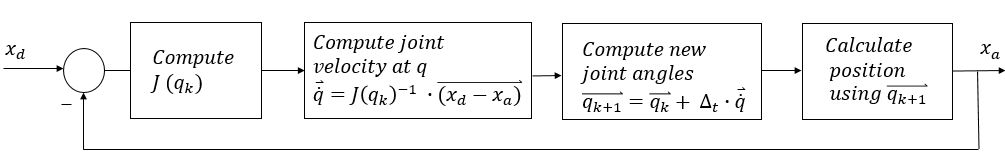
\includegraphics[width=\linewidth]{Newton-Raphson_loop.jpg}
\caption{The Newton-Raphson Method applied to Inverse Kinematics}
\end{figure}
\end{center}

V-REP uses this approach for its inverse kinematics solver; except with the Pseudo-Inverse Jacobian, as it intrinsically provides the smallest 2-norm among all solutions, even when the arm is near singularities. When a set of joints is in inverse kinematics mode, either the Pseudo Inverse or Damped Least Squares method can be chosen, with an iteration number. This iteration number is the number of times V-REP will perform the above loop before using the evaluated change in angles to move the joints. Thus, the number of iterations determines the accuracy of these methods, where the more iterations the more processing time is required to narrow down on a more accurate solution.

\begin{center}
\begin{figure}[htb]
  \includegraphics[width=0.5\linewidth]{VREP_ik_dialog.jpg}
\caption{The calculation method for Inverse Kinematics in V-REP}
\end{figure}
\end{center}

Due to V-REP's knowledge on the position of joints within a serial chain, using the inbuilt D-H solver the transformation matrix for the arm is determined. Thus, from this the Jacobian, and then the Pseudo-Jacobian matrices are computed for a given configuration, and used to calculate the change in angles required for the `Tip` object to reach the `Target` object; given a solver type as specified above. This method will be mimicked in this thesis such that the client program can have the ability to control the joint angles of both V-REP and the physical Kinova Jaco arm.

\chapter{Design Approach}

This chapter looks into the design of the client program, the decisions and functionality required to complete the program's objectives. Firstly the overall objectives are defined, and then the procedures for completing these are provided. The results chapter will go into detail of how the functionality was implemented, and the successes and failures which arose.

\section{Client Program Functionality Requirements and Design}
Using V-REP's remote API, a client program is required to be developed to allow the external control of the virtual Jaco arm. This program must have the following functionality:

\begin{itemize}
	\item Be able to control a scene with the Jaco arm with joints either in Forward or Inverse Kinematics modes
	\item Allow input commands come from the user's keyboard, or from an external joystick
	\item Allow the control of the Jaco arm by calculating its own inverse kinematics
	\item Be able to connect to V-REP through a specified IP address and port number
	\item Be easily able to convert between implemented kinematics modes
	\item Have data-steaming functionality to enable collision detection
	\item Be able to quickly retrieve the object handles for the joints of the Jaco arm, for any given V-REP scene before processing
	\item Be able to identify when the Jaco arm is in an undesirable configuration and have automatic adjustments; an undesirable configuration is when the gripper is facing upwards, as if to grab something from above, instead of out in front.
	\item Allow real-time manipulation of the virtual robotic arm and V-REP scene
\end{itemize}


Considering there was a distinct lack of background experience with V-REP and using remote API's, the development of the client program was broken down into small stages. These stages together allowed the full development of the program:

\begin{enumerate}
  \item Import the Jaco arm into V-REP, add the gripper; additionally, learn how to import models into the scene and create a robotic arm for the interest of familiarising oneself with V-REP
  \item Use a familiar coding language to interface with the remote API to communicate with V-REP
  \item Determine a method for getting the object names within the scene, to make a mapping between object handles and object names (i.e. it is known that the fourth joint's name will contain the word 'joint' and the number 4, but that doesn't give a way of communicating with V-REP, as the remote API requires object handles.
  \item Make the IP address, port number, and scene mode input arguments to the program for quick management
  \item Develop the client program to be able to send and receive joint angles from the Jaco arm in V-REP
  \item Create an interface for communicating with the client, to be able to transfer input commands to the client; for getting and moving joint angles
  \item Create a V-REP scene with the Jaco joints in Inverse Kinematics Group, such that the end-effector tracks a target object
  \item Using the mapping for object names to object handles, get the target and tip objects' handle
  \item Control the position of the target during a simulation, so the Jaco arm follows the commands.
  \item Design an interface for giving keyboard inputs to move the target in the scene
  \item Find a way of getting the input from a gaming controller via USB; i.e. 'X' button pressed.
  \item From a separate program, create a child process to run the program for getting the controller inputs, and send them to the parent process
  \item Integrate this functionality into the V-REP client program, so when the scene mode is Inverse Kinematics, the joystick application process is created and communicates with the client of any input changes.
  \item Using MATLAB, form the forward and inverse kinematics solutions using the D-H parameters, analytical inverse method, a control system for reducing angle error using regulators, and the Jacobian matrix for a given position
  \item Adjust the tip dummy object to mimic the end-effector position from the forward kinematics
  \item Integrate forward kinematics functionality into the client program
  \item Integrate the analytic inverse solution into the client program
  \item Integrate the control scheme solution into the client program
  \item Integrate the jacobian inverse method into the client program
  \item	Tune the solutions individually
  \item Devise a method of quickly swapping between inverse kinematics solutions
  \item Optimize the code and program

\end{enumerate}

Through the development of the program, additional stages were added, such as enabling the child process terminate when there wasn't a joystick connected, and allowing the program to then accept inverse kinematics commands through keyboard input. Later, it was discovered that threads cause blocking of other tasks, and shouldn't be kept running. These additional developments will be outlined in the approach section below, as the development of the program is explained. 

\section{Project Development}

\subsection{Set Up}
Originally, the program was written in python as it allowed easy manipulation of variables, and passing of information to V-REP. There is plenty of example code for setting up a connection to V-REP from a python program. This allowed an understanding of how the connection was established; V-REP needed to be set to read from a given port, and then from the client program, a call to connect was made which returned a client identification number, which is used for every interaction thereafter. In the python version, a call to 'import vrep' was made, which handles the remote connection and allows the use of the python library. The script was really basic, it created a connection, got the object handles given the name of the joints of interest, set some parameters and moved the joints. This process is descibed by the figure below.


\begin{center}
\begin{figure}[htb]
  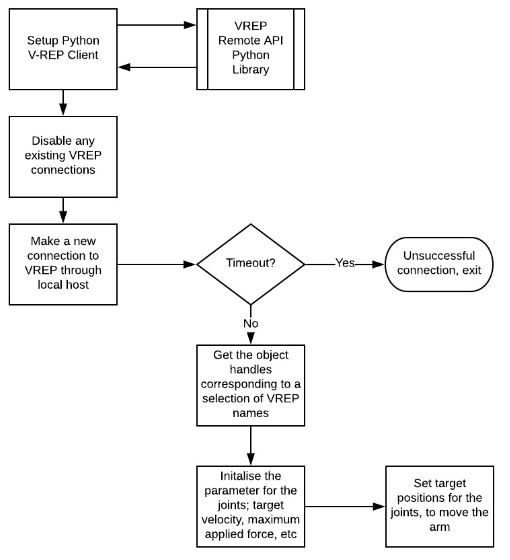
\includegraphics[width=0.8\linewidth]{python_flow_diagram.jpg}
\caption{Simple V-REP client program in Python Flow Chart}
\end{figure}
\end{center}


At this stage, a better definition of the problem scope was provided by Dr Singh, which included many different ideas than that expected. Dr Singh made mention of having the scene in V-REP be projected onto a table using a homography, and then interacting with the virtual arm by moving in-front of the projection. From this, I began to add sensors and cameras into the V-REP scene, so a fixed point can be projected; significant delay came with the addition of a camera in the scene whilst moving the arm, and thus this design concept wasn't pursued further. The inclusion of a joystick also became a requirement for this task, in that the end-effector of the arm should be controlled with a joystick. From this, it was decided that to allow interfacing with peripherals, the client program should be written in C. The idea behind this was that an executable can create child processes that are separate to the VREP client, which handle tasks such as reading from the joystick, or projecting the environment onto a table (if that was to be required).

From previous studies, it was known how to develop a C application in the Linux environment, and thus a virtual machine was made. The program was then rewritten in C, which had it's own problems associated with including the external API files in the correct order, and the generation of the makefile; there was limited instruction on which of the many files should be included. The makefile is depicted in the image below for documentation purposes.


\begin{center}
\begin{figure}[htb]
  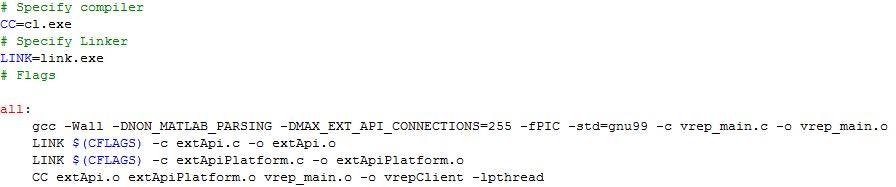
\includegraphics[width=1.1\linewidth]{makefile.jpg}
\caption{V-REP Client Makefile}
\end{figure}
\end{center}


The client then became under development, with the first task being to extract the object names and handles from V-REP. Unfortunately there wasn't a remote API function for getting object names, however there was one for handles. Thus, an internal V-REP function needed to be created to return object names given an object handle. This was done in the V-REP main script, and was called in the remote API using the simxCallScriptFunction(). This remote API function expects 4 types of information to be returned from V-REP, (an integer, float, string and a buffer), thus the Lua function returned two empty tables, one containing the object name, and an empty buffer. Using the blocking communication technique, this function was able to be called for each object handle in the scene, and the name stored.

\begin{center}
\begin{figure}[htb]
  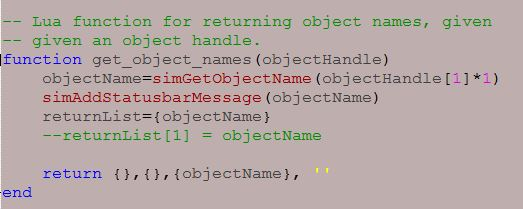
\includegraphics[width=0.8\linewidth]{object_names.jpg}
\caption{Lua function in V-REP main for retrieving object names}
\end{figure}
\end{center}

This process caused a slight delay on start up, whilst the client program retrieved the names corresponding to important joints of the Jaco arm, and mapping them to their respective object handles; all of the information for objects in the V-REP scene were stored in an struct. Thus, it was desirable to write the mapping for a regularly used scene to a text file once it is retrieved from V-REP, allowing the text file to be used on start-up instead of communication to V-REP when the simulation is run again. To further develop this, the client program will look for a given text file for a scene, and if it does not exist it will get the information from V-REP, and write it to the file for next time; otherwise it will fill the struct with the information from the text file. As the important information from V-REP is the names and object handles of joints, motors and the Target object, this is the only information saved to the file, making it a much faster avenue than requesting from V-REP and sorting.

\vspace{\baselineskip}

\begin{center}
\begin{figure}[htb]
  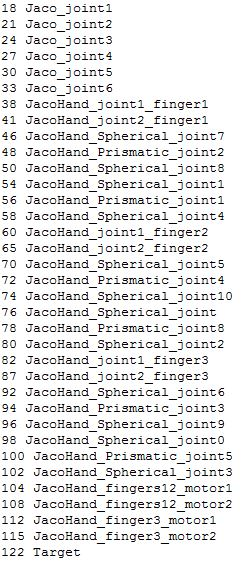
\includegraphics[width=0.4\linewidth]{text_file_example.jpg}
\caption{Example of a text file created by the V-REP client}
\end{figure}
\end{center}

\vspace{\baselineskip}

Now that the client program was able to get the joint handles in the scene, and send desired joint positions. Merging this functionality together, the client became able to automatically associate a joint number with an object handle and then set or get the joint angle from V-REP. To further progress this, the command-line interface was developed to take in forward kinematics inputs, of the form, `joint number` `angle to move`, with enter being used to store the request. From this, the program was able to set a joint angle of the Jaco arm in V-REP, and return the new angle. This process is outlined below.

\vspace{\baselineskip}

\begin{center}
\begin{figure}[htb]
  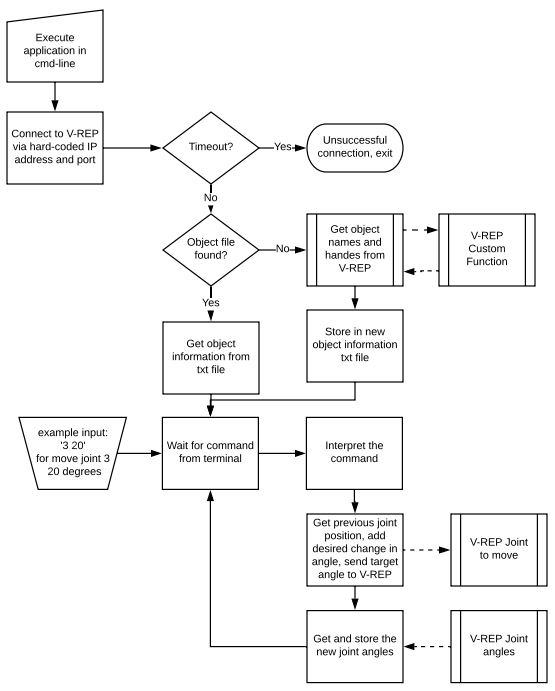
\includegraphics[width=\linewidth]{client_fk.jpg}
\caption{Client program in Forward Kinematics mode}
\end{figure}
\end{center}

\vspace{\baselineskip}

From this, it was important to ensure the forward kinematics can be calculated, to ensure the Jaco arm's end-effector position was in the expected position when returned from V-REP. Furthermore, it would be required for the inverse kinematics derivation and implementation. 

\subsection{Forward Kinematics Implementation}
% forward kinematics
Kinova Robotics supplied documentation that assisted with the forward kinematics of the arm. In their $JACO^2$ 6 DOF Advanced Specification Guide, is the D-H parameters, joint lengths and offset angles for the robotic arm. Expressed in the table below are the numerical values for the D-H parameters, for the given axis positions along the arm. It can be seen that the axis for joint 4 isn't at the physical motor position, rather at the angled point in the link, this is to simplify the parameters as is at the bend, pointing towards joint 3, and is merely powered by the motor at joint 4. This occurs again at joint 5, where links 4 and 5 have a bend of 60 degrees, moving the axis of rotation away from the joints. The parameters used in this case are the 'Classical D-H Parameters' from the Kinova documentation, however there are other sets of parameters for the Jaco arm. For instance, the zeroth axis can be turned such that $\alpha_0$ is 0, and similarly for $\alpha_3$, where $\alpha_2$ and $\alpha_4$ can be $-pi/2$. The classical parameters were used as it matches the Jaco documentation, Peter Corke's Robotic Toolbox, and the set of angles to make the arm stand straight up could be easily determined. 

\vspace{\baselineskip}

\begin{center}
\begin{figure}[htb]
  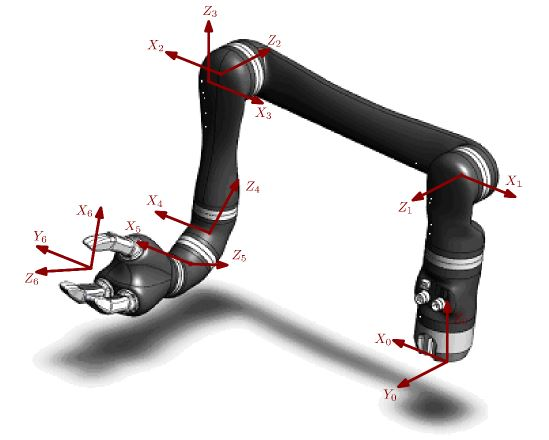
\includegraphics[width=0.7\linewidth]{jaco_axis.jpg}
\caption{D-H Parameters axis for each joint on Jaco arm}
\end{figure}
\end{center}

\vspace{\baselineskip}



\begin{center}
\begin{table}[htb]


    \begin{tabular}{| l | l | l | l | l | p{15cm} |}
    \hline
    Joint & $\alpha_{i-1}$ & $a_{i-1}$ & $d_i$ & $\theta_{i}$ \\ \hline
     1 & pi/2 & 0 & 275.5 & q1 \\ \hline
     2 & pi & 410.0 & 0 & q2 \\ \hline
     3 & pi/2 & 0 & -9.8 & q3 \\ \hline
     4 & pi/3 & 0 & -250.08 & q4 \\ \hline
     5 & pi/3 & 0 & -85.563 & q5 \\ \hline
     6 & pi & 0 & -202.78 & q6 \\ \hline
    \end{tabular}
    \caption{V-REP remote API operation modes}
\end{table}
\end{center}

\vspace{\baselineskip}

Using the theory outlined for deriving the end-effector position from a set of joint angles (forward kinematics), the transformation matrix in terms of symbolic joint angles $\vec{q}$ for this arm was calculated using MATLAB. The script for this is provided with this paper, where it can be seen that the transformation matrix is denoted by the variable A. From the figure of the Jaco arm provided, it can be seen that it is in folded over position, whereas in V-REP the Jaco arm begins in a straight up configuration. Thus, there is a difference between the mapping for angles in V-REP compared to the transformation matrix, meaning, for them to be transparent the angles of the transformation matrix need to be offset to mimic that of the virtual arm. Correctly, for the transformation matrix to provide an arm configuration with the gripper at it's tallest point, like V-REP, the angles need to be substituted into the transformation matrix as;

\vspace{\baselineskip}


$\vec{q} = [ pi, pi/2, -pi/2, 0, -pi, pi]^T$

\vspace{\baselineskip}


resulting in an end-effector position;

\vspace{\baselineskip}


$\vec{X} = [0, -64.299, 1181.145]^T$

\vspace{\baselineskip}


Thus, for changes in joint angles relative to V-REP's starting position, the following substitution had to be made;

\vspace{\baselineskip}


$\vec{q} = [ pi - q_1, \frac{pi}{2} + q_2, -\frac{pi}{2} + q_3, q_4, -pi + q_5, pi + q_6]^T$

\vspace{\baselineskip}

Thus $q_i$ is the offset in angle between one joint and the next, as per the forward kinematics convention provided in the theory section of the report. To separate the V-REP communication and terminal input handling to the mathematics associated with forward and inverse kinematics, functions for these were placed in its own kinematics files (called kinematics.c/.h). Once the forward kinematics solution was correct in MATLAB, the mathematics that described the end-effector position in terms of joint angles was inserted into the file, and given an input command that ran the function and printed the expected end-effector position. This was able to prove that the forward kinematics model and the tip position agreed; after some slight tweaking of the tip position relative to joint 6.


\subsection{V-REP Inverse Kinematics}
After the forwards kinematics was correct, the inverse kinematics methods can be written in MATLAB and derived, to be integrated into the client program. For the integration, the client program had to be set-up to take inverse kinematics inputs, and manipulate the joint angles with V-REP accordingly. In addition to this, the client program needed to be able to control the target object in a inverse kinematics V-REP scene. Thus, the next objective to complete was to get V-REP to recognise the Jaco arm serial chain and compute the joint angles such that the tip follows the target, moved by the client program.

This part was straight forward, an 'IK Group' needed to be created that contained the Target and Tip objects, and the reference frame to be set to that of the Jaco's base. The solver can have constraints on the x, y, z, $\theta_x$, $\theta_y$ and $theta_z$; thus the tip can be constrained to the target's position and orientation. The desired precision can also be specified, which is how close the solver's solution can place the tip to the target's position before finishing the interations (before the maximum iteration number is reached). The settings chosen where 0.5mm in translational coordinates, and 0.1 radians for the angles, no restriction on $\theta_z$ so the arm always points away from its base, and a maximum number of steps to be 5. The Damped Least Squares solver was selected with damping of 0.052, this provided a smooth transition towards a desired path; whereas the Pseudo Jacobian Method can have significant error around the target before getting a precise enough approximation, causing scattered movements. More specifically, for a small change in tip to target position of 1.5mm in the y, and 7.6mm in the z, the Pseudo Jacobian method with 5 (and even 50) iterations wasn't able to change the base angle enough for joint 2 and 3 to move into the correct plane to allow the error in y and z be limited. This problem has occurred as V-REP has the Jaco model placed up-right, thus there are singularities with joints 2 and 3 being aligned. The Damped Least Squares method performs better close to singularities, where 5 iterations in this mode can effortlessly move the end-effector into position. Below is a figure presenting the Jaco arm in inverse kinematics mode with small error in target to tip position. Following is a figure of the results between using the DLS and Pseudo inverse methods. Due to the arm being in inverse kinematics mode, the joint angles cannot be set to place them out of singularities on start up; as V-REP is constantly trying to make the target and tip error fall below the threshold.


\begin{center}
\begin{figure}[htb]
  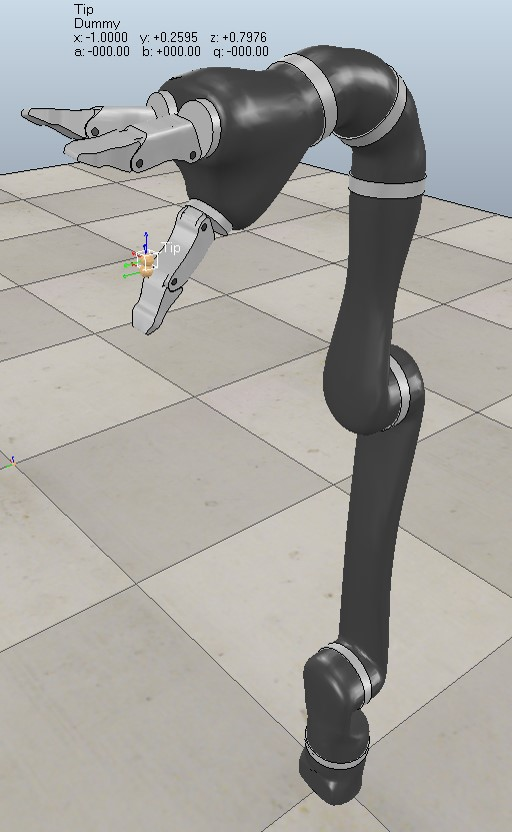
\includegraphics[width=0.4\linewidth]{Small_change_jaco.jpg}
\caption{The Jaco arm in V-REP with joints set to IK mode, with a small error in target to tip position}
\end{figure}
\end{center}


\begin{center}
\begin{figure}[htb]
  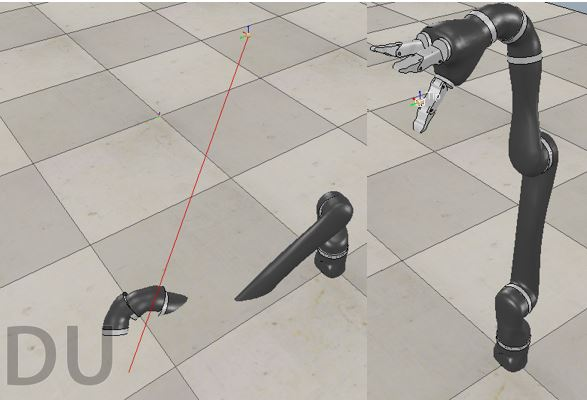
\includegraphics[width=0.9\linewidth]{Small_change_jaco_result.jpg}
\caption{Left: the Jaco arm using the Pseudo Inverse Jacobian with 50 iterations. Right: the Jaco arm using DLS of damping 0.05 and 5 iterations}
\end{figure}
\end{center}


For this robotic manipulator it was found that the DLS method was the best to used with V-REP, and the small iteration number didn't come with any noticeable delay in the program; thus satisfying the real-time objective.

The client program was set up for interpreting inverse kinematics inputs, being keyboard commands. Given the command, presented in the table below, the target position will be retrieved from V-REP, incremented on according to the command, and then the world position of the target would be reset; moving the arm.

\begin{center}
\begin{table}[htb]

    \begin{tabular}{| l | l | p{6cm} |}
     \hline
     Keyboard Command & Change in Tip Position & Description  \\ 
     \hline
     'w' & 3 mm & radially out (horizontal) from the base of the arm \\ 
     \hline
     's' & 3 mm & radially in (horizontal) towards the bass of the arm \\ 
     \hline
     'a' & 3 mm & anti-clockwise (horizontal) from the current tip position \\ 				 \hline
     'd' & 3 mm & clockwise (horizontal) from the current tip position \\ 
     \hline
     '-' & 3 mm & change in height of the tip downwards \\ 
     \hline
     '+' & 3 mm & change in height of the tip upwards \\ 
     \hline
    \end{tabular}
    \caption{Client program IK input commands}
\end{table}
\end{center}

\vspace{\baselineskip}
The maths for calculating the new coordinates of the target were quite simple, where $\vec{P_t}$ denotes the position of the tip relative to the base such that;

\vspace{\baselineskip}
$\vec{P_t} = \vec{Tip_{worldCoorinates}} - \vec{JacoBase_{worldCoordinates}}$

\vspace{\baselineskip}
the 'w' command would have the following computations;

\vspace{\baselineskip}
$radius = \sqrt{P_{t_x}^2 + P_{t_y}^2}$

\vspace{\baselineskip}
$radius = radius + \Delta radius$

\vspace{\baselineskip}
$angle = atan2(P_{t_y}, P_{t_x})$

\vspace{\baselineskip}
$P_{t_x} = radius \times cos(angle)$

\vspace{\baselineskip}
$P_{t_y} = radius \times sin(angle)$

\vspace{\baselineskip}
It was found that the program could seamlessly control the target in V-REP,and the end-effector would follow.

\subsection{Joystick Integration}
The next objective was to add a joystick as an input source for moving the end-effector. It was assumed that the physical Jaco arm would be set-up to a Windows computer in the Robotics Design Lab at UQ, and as a port is necessary for creating a processes from the client program to read the joystick, it was decided that the client program was required to be developed on a Windows computer; rather than a virtual machine were it cannot directly access USB ports. The task of moving to Windows was time consuming, Linux compilers were first downloaded to Windows such that the program can compile in command-line. Unfortunately the networking on Windows is different to Linux, and so there wasn't libraries for converting Linux network code to a form understandable by Windows. It was decided that a new client program should be created in Visual Studio, and then the client program's custom files have the code copied over.

%https://www.libsdl.org/download-2.0.php
Only Windows has the ability to control the Human Interface Drivers, however the Windows API allows one to communicate with this via functions such as GetRawInputData(); available with hidsdi.h. Unfortunately a program using Windows API can only communicate with another Window through Window messaging (queues). The client program was a console application, which had the ability to communicate with other applications through a method similar to piping in Linux. Given it was desirable to find an existing joystick interface as an executable which can easily be run by a creating a child process, many platforms were tested to determine the easiest to interface with. The notes taken during this time is provided in the appendix, where Windows API, HTML Gamepad API, LibUSB, and Simple Directmedia Layer (SDL) source code were tested. It was found that SDL provided the best means in interfacing with the Joystick, as the library offered the source code that was editable from Visual Studio. Initially the project, testjoystick, was designed to display information about the joystick, and show which buttons were being pressed in a Window. It was also discovered that the application had it's own handle to the console, using SDL\_log to print to terminal. This meant that usual handles to the terminal such as stdout and stdin had no effect on the console window. Thus, changes were made to the program (it should be noted that SDL is open-source as long as it's referenced and changes made are commented on);

\begin{itemize}
	\item The code that created and controlled the window was removed; so the application only printed to the control via SDL\_log
	\item The handle to stdout and stdin were redefined; such that stdin pointed to the STD\_INPUT\_HANDLE, which was opened for reading.
	\item The code was made to print to stdout "No Joysticks Attached" and exit; so the child process isn't left open when there isn't a joystick.
\end{itemize}

%https://msdn.microsoft.com/en-us/library/windows/desktop/ms682425(v=vs.85).aspx
A new project was made to attempt to spawn a child process using the Microsoft Developer Network (MSDN); libraries accessible from Visual Studio. With reference to the example code on the CreateProcess function, information successfully flowed between the testjoystick application and the new project file. This code was then copied into the client program, in the file joystick.c. This file was used to store all code relevant to the joystick, such as creating the process, reading from the process, interpreting the button presses and joystick positions, adding the relevant information to the input buffer, and the handing of passing commands from the buffer to the main client thread. A total of 3 threads were used, with two made to service the commands of the joystick;

\begin{center}
\begin{table}[htb]
    
    \begin{tabular}{| l | p{10cm} |}
    \hline
     Thread & Description     \\
     \hline
     Main & Handled input commands from the joystick buffer or from the terminal, and communicated with V-REP to produce the desired outcome  \\
     \hline 
     Joystick Interpretation & Reads from stdout of the joystick process, interprets the information, and adds a (w/s/d/a/-/+) command to the joystick command buffer with decimal value corresponding to the amount that the joystick was pushed for that command (0 for no press, 1 for 100\% pressed).\\
     \hline
     Joystick Add Command & This task keeps track of the last command to be added to the buffer, when the push value is greater than 0, and 750ms has passed, a copy of the last command is added to the buffer as the joystick is still pressed down. \\ \hline
    \end{tabular}
    \caption{Client program IK input commands}
\end{table}
\end{center}


It can be seen in the below figure that the output of the joystick process (SDL\_log prints that were provided, but same information that is sent to the client program) shows the axis being toggled as a number between 0 and 3 (two axis per joystick) with 16-bit signed integer representing the amount it's pushed on that axis. Thus, when a joystick axis is held and not returned to zero, the output of the joystick process only shows that it's reached 32797, but doesn't keep printing to show that it's still held there. For this reason an additional thread was created to check the joystick buffer, and re-add commands after a period without change. It was found that 750 ms was the optimal time to wait between adding to the buffer, as it took on average 600 ms for a command to be interpreted sent to V-REP. This average is CPU speed dependent, and thus changes from computer to computer; it is similar to the sensitivity of the joystick.

\begin{center}
\begin{figure}[htb]
  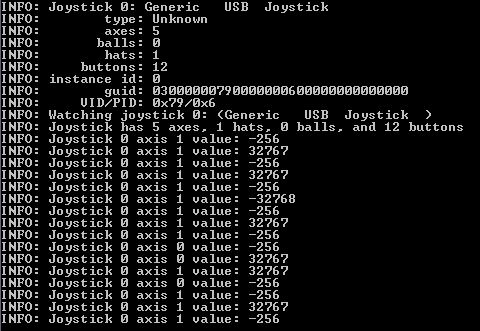
\includegraphics[width=0.9\linewidth]{joystick_cmdline.jpg}
\caption{An example of the terminal output of the joystick process when the left joystick is toggled on}
\end{figure}
\end{center}

With the joystick successfully moving the tip position in V-REP, the main objective of having an external tool control the robotic simulation was complete. It was now a manner of getting different inverse kinematics methods working with the V-REP client program. This was to enable the V-REP scene can be in forwards kinematics mode, and the client program move the joint angles to provide a desirable end-effector position. The chosen methods for the client program were, the analytical approach as this would require the least number of calculations, a control systems approach, and using the inverse Jacobian with Newton-Raphson's method. Three were chosen to determine which was the best given the design objectives.

The client program was further developed during this stage, to incorporate commands for getting the world coordinates of objects, pausing communication between V-REP and the client to allow all joint angles to be sent at one time, streaming mode was trialled with the objective of updating the client's knowledge of the joint angles, and setting up the interface having a forward kinematics scenes with inverse kinematics inputs, and a way of quickly flicking between the different inverse kinematics solutions.

\chapter{Kinematics Approach}
\section{Forward Kinematics}
As aforementioned, the forward kinematics was derived using the D-H Parameters provided by Kinova and by following the theory section of this report for the transformation matrix. Due to the amount of symbolic expressions, MATLAB didn't ignore numbers close to zero. Thus, before using the transformation matrix, each coefficient in each index was filtered and extracted if it was smaller than 0.000001. The matrix expressions are still too long to be displayed here, however it is available in an attached MATLAB scripted titled forwardKinematics.m and in the kinematics.c file for the client program. It was found that the transformation could accurately determine the position of the end-effector given a set of angles; this can be checked by typing 'fk' as an input command for the client program, and checking the coordinates of the tip object in V-REP.

\section{Inverse my Matrix Manipulation}
In order to take the strain off V-REP doing all the computations, and to give the control of either forward or inverse kinematics control to the client program, three inverse kinematics methods were integrated into the client program. The first attempt at an inverse kinematics solution was to derive the relationship between joints through manipulations of the transformation matrix, such that;

$(A_{0}^{1})^{-1} T = A_{1}^{2} A_{2}^{3} A_{3}^{4} A_{4}^{5} A_{6}^{6}$

After rearranging the matrices between the left and side and right hand side, and inspecting the indexes of both sides for equalities, no fruitful results were found. For instance, when observing the results of both $A_4^5 * A_5^6$ compared to $(A_0^1 * A_1^2 * A_2^3 A_3^4)^{-1} A$, each index of both matrices were mathematically identical; any variances could be corrected with trigonometric identities. 

\section{Inverse by Analytical Approach}

To begin this approach, the Jaco arm was redrawn in different configurations to determine how the varying each joint can change the end-effector position. Following the approach outlined in the theory section of this report, it can be seen that the second link forms a triangle with point $\vec{P}$, formed by the joint angles $q_2$, $q_3$ and the joining joint lengths. An angle of 60 degrees is always present between the rotational axis of $q_4$ and link $\vec{PR}$, similarly with $q_5$ and link $\vec{RS}$. In the figure provided, $q_4 = \frac{\pi}{2}$ and $q_5 = \pi$, which leads to the end-effector remaining in the x-z plane; the angles contribute no y-component. 

\begin{center}
\begin{figure}[htb]
  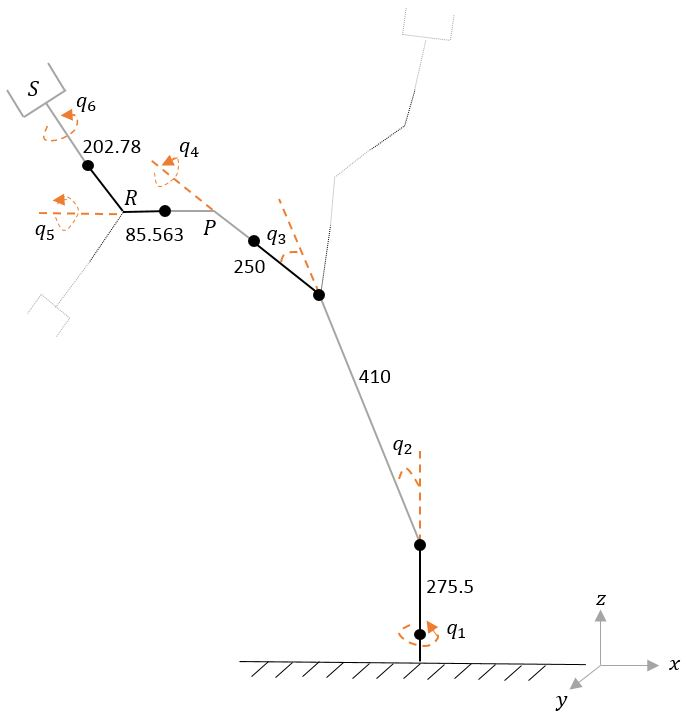
\includegraphics[width=0.9\linewidth]{jaco_angles_figure.jpg}
\caption{Dimensions and angles of Jaco Arm}
\end{figure}
\end{center}

Varying these two angles in any means will result in a decrease in angle visible in this figure between the rotational axes and the links; as part will form into the y-z plane. This leads to the figure below, where these angles are denoted $\alpha$ and $\beta$ respectively. Instead of considering point $\vec{P}$, the axial coordinate due to the 60 degree links were added to the link prior, moving point $\vec{P}$ to $\vec{P'}$.

\begin{center}
\begin{figure}[htb]
  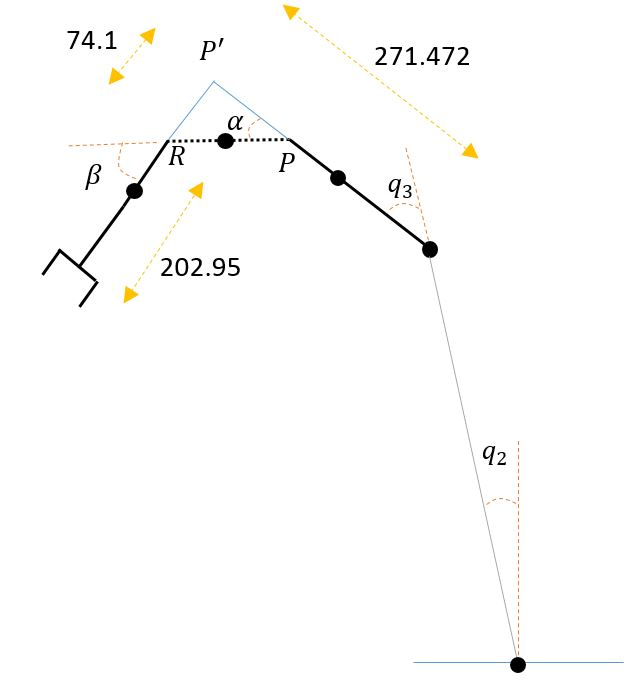
\includegraphics[width=0.8\linewidth]{jaco_inv_figure.jpg}
\caption{Simplification of Jaco arm geometry}
\end{figure}
\end{center}

Limiting $\alpha$ and $\beta$ to 60 degrees, results in the following relationships;

$\alpha = \frac{q_4}{6}$

$\beta	= \frac{q_5 - \frac{\pi}{2}}{6}$

Focusing more on the wrist, the lengths of the proposed vectors can be determined; note that $D_4$ and $D_5$ are known from the D-H parameters of the arm.

\begin{center}
\begin{figure}[htb]
  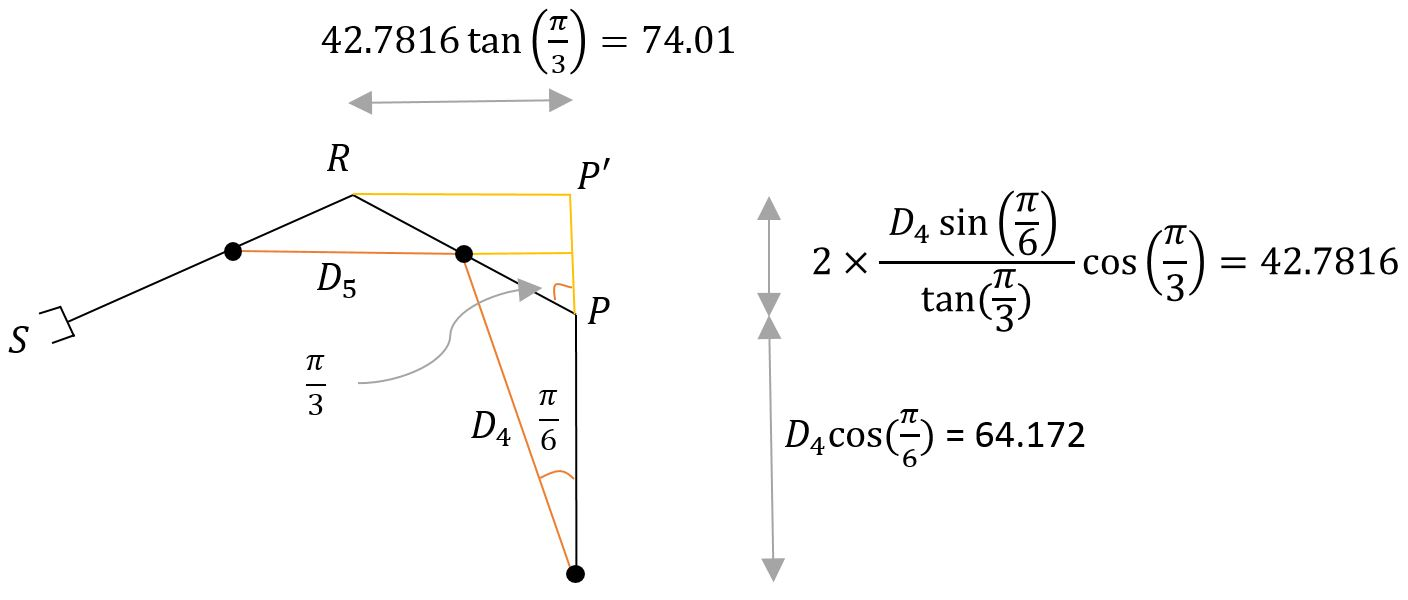
\includegraphics[width=0.9\linewidth]{jaco_inv_wrist_figure.jpg}
\caption{Simplification of Jaco arm wrist geometry}
\end{figure}
\end{center}


From this figure it was found that $\vec{PR} = 85.563$

The point R can thus be written in terms of point P' and the affect of the arm angles contributing length in the x-z plane such that;

\vspace{\baselineskip}

$R_x = P_x + 85.563 sin( q_2 + q_3 + \alpha)$

$R_y = P_y + 85.563 sin( q_2 + q_3 + (\frac{pi}{3} - \alpha))$

$R_z = P_z + 85.563 cos( q_2 + q_3 + \alpha)$

\vspace{\baselineskip}

Similarly for the end-effector position $\vec{S}$ in terms of $\vec{R}$

\vspace{\baselineskip}

$S_x = R_x + 202.95 sin( \beta + \alpha + q_2 + q_3)$

$S_y = R_y + 202.95 sin ( (\frac{\pi}{3} - \beta) + (\frac{\pi}{3} - \alpha) + q_2 + q_3)$

$S_z = R_z + 202.95 cos( \beta + \alpha + q_2 + q_3)$ 

\vspace{\baselineskip}

From the theory section, it is known that;

\vspace{\baselineskip}

$P_{xy}^2 + (P_z - D_1)^2 = 410^2 + 250^2 - 2 \times 410 \times 250 \times cos(q_3)$

$\rightarrow q_3 = cos^{-1} ( \frac{P_{xy}^2 + (P_z - D_1)^2 - 410^2 -250^2 }{2 \times 410 \times 250}$

\vspace{\baselineskip}

and,

\vspace{\baselineskip}

$cos(q_2) = \frac{ P_{xy} (410 + 250 sin (q_3)) + 250 sin(q_3)(P_z - D_1) }{410^2 + 250^2 + 2 \times 410 \times 250 cos(q_3)}$

$sin(q_2) = \frac{-P_{xy} \times 250 sin(q_3) + (P_y - D_1)(410 + 250 cos(q_3))}{410^2 + 250^2 + 2 \times 410 \times 250 cos(q_3)}$

$\rightarrow q_2 = atan2( \frac{sin(q_2)}{cos(q_2)})$

\vspace{\baselineskip}

The angular position of $\vec{P}$ in the x-y plane is dependent on $q_1$, and the radial position from the base in x-y coordinates is dependent on the angles of $q_2$, $q_3$, as seen above. Thus, the expression for $q_1$ in terms of $\vec{P}$ will have the form (a constant offset of angle occurs do to the arm's orientation in V-REP);

$q_1 = atan2( P_y, P_x)$

Therefore, given a desired position for $\vec{P}$, joint angles $q_1$, $q_2$ and $q_3$ can be determined. From this position and a known end-effector position, $\vec{S}$, the angles $\alpha$, $\beta$, can be determined and thus $q_4, q_5$;

Substituting out $\vec{R}$, it is known that;

$sin(q_2 + q_3 + \alpha) 85.563 + P_x = S_x -202.95 sin(\beta + \alpha + q_2 + q_3) $

This can be repeated for the y and z coordinates, however it can be seen that the relationship between $\vec{P}$ and $\vec{z}$ depends on all the angles being known, or, both $\vec{P}$ and $\vec{S}$ being known; not only $\vec{S}$ unless $\alpha$, $\beta$, are known, or more relationships between the joints are found. This is not a dead-end however, as it is known that the relationship between $\vec{P}$ and $q_1$, $q_2$ and $q_3$ exists, and if $\alpha$, $\beta$ are static between movements, it can be found that;

$\Delta \vec{P} \propto \Delta \vec{S}$

thus, knowing the change in position required at the end-effector, the change in coordinates of $\vec{P}$ can be approximated to move the end-effector to the desired position. Discrepancies will depend on the angle of the arm joints, however this method will bring the end-effector close to the desired point. Any variation in position can be corrected using feedback control on the approximated angles $q_2$, $q_3$, calculated as per the above formulas. Below is a figure presenting the controller that was designed;


\begin{center}
\begin{figure}[htb]
  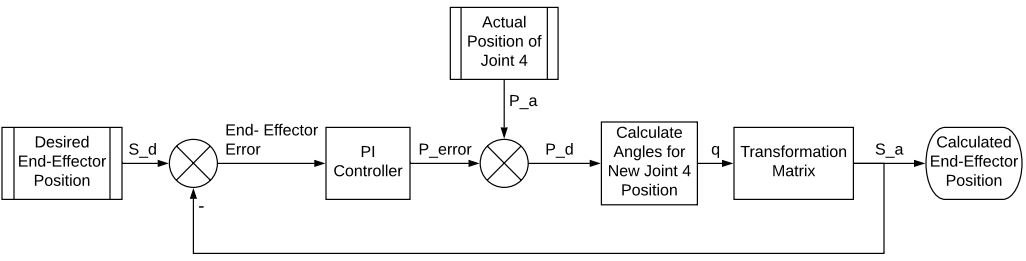
\includegraphics[width=1.14\linewidth]{inv_kinematics_and_control.jpg}
\caption{Control loop for approximating the joints angles to move the end-effector using the position of the fourth joint}
\end{figure}
\end{center}

The controller gains are smaller than 1 to reduce the error being added to the position of the fourth joint, such that a solution is approached with each loop iteration. Integral control allows the error to be added with each loop, reducing steady state error, whilst the proportional gain allows the required state be reached quickly.

In the MATLAB script, inverseKinematics.m, the steps for calculating the required angles for a desired end-effector position is presented; following the maths presented above. After verification of this process, the code was written in the client program to tune the gains of the controller, and add any angle offsets present between theoretical calculations and the joints of the arm in V-REP. The PI controller was able to be tuned by writing the calculated end-effector position to a spread sheet (stored in programming/client/x62/Debug) each loop iteration; allowing the plotting to view the response. For this design, an accuracy of 6mm in each component of $\vec{S}$ was required, with a maximum loop iteration of 20. It was decided that the $K_P$ and $K_I$ gains for each axis should be equal, as it is desirable for the arm to weigh each axis equivalently. The response with the lowest overshoot and steady-state error was found to have gains of $K_P = 0.08$ and $K_I = 0.2$, with the response of each axis being presented below; and further in the appendix. It can be seen that the responses converge to the desired values in practice. In code, bounds were placed to ensure the control loop was not forcing the arm to reach an unreachable end-effector position.

\begin{center}
\begin{figure}[htb]
  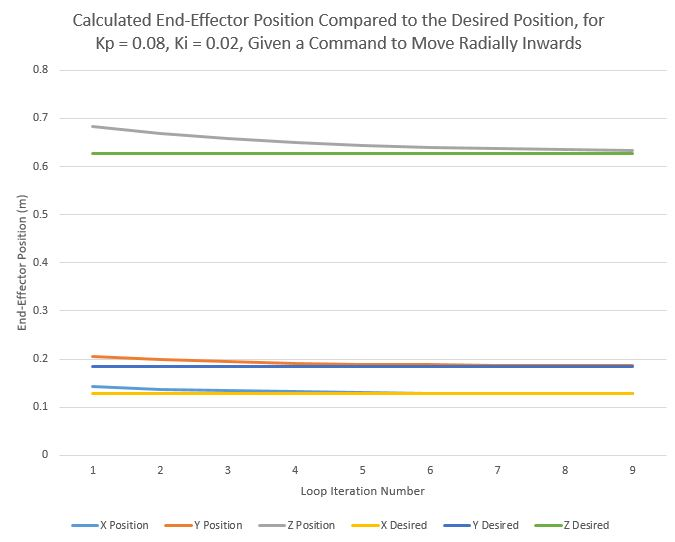
\includegraphics[width=1\linewidth]{des_act_inv1_plot.jpg}
\caption{Response of Chosen Controller Given a Change in End-Effector Position Command (3mm in the x-y plane)}
\end{figure}
\end{center}

\section{Inverse by Control Loops}
The success in the former section called for a trial of using control loops to govern the change in angles required for reducing the error in end-effector position. A key problem with this form of control is that there is no method of checking for undesirable joint configurations; such as the arm folding onto itself. Due to this system being non-linear, the controller response will depend on position, and thus will only be used for correcting small errors in end-effector position. In MATLAB Simulink the original model was created, where the inputs were the desired end-effector coordinates. To give the system a localized approximation, the first 3 angles were calculated using the inverse kinematics described in the previous section. To make a start, the 6 joint angles had a PI controller with proportional gain being a fraction of their following link lengths. The purpose of this was that, for example, the second link is the longest at 410mm, and thus small angles of $q_2$ will effect the end-effector position more than $q_3$, which moves a link of length 200mm; thus the gains for controlling $q_3$ are more than that for $q_2$. The error being corrected was not the difference in x, y, z coordinates between the desired position $S_d$ and actual position $S_a$ of the end effector. Instead, the change in angle between these locations in the x-y plane, and ground-z plane were used; this was to decrease the probability of having inaccurate error from changing between quadrants. The use of angles also limits the error to between 0 and $2\pi$, which is the same range as the angles for the robotic arm, whereas if displacements were used the error would be linear and large, differing significantly to joint angles. The angular displacement error, $\theta_z$, $\theta_{xy}$ are illustrated in the figure below.


\begin{center}
\begin{figure}[htb]
  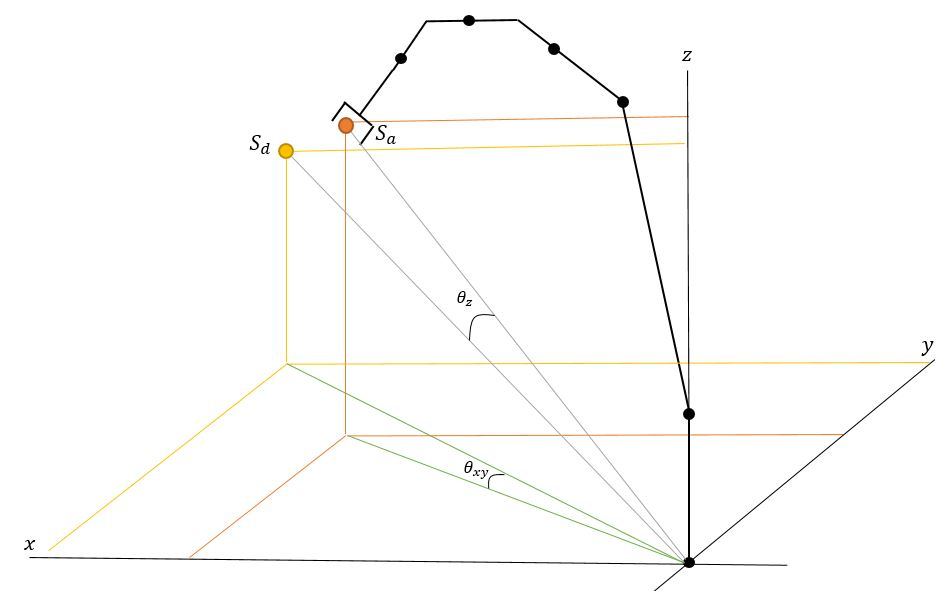
\includegraphics[width=1\linewidth]{jaco_inv_control_figure.jpg}
\caption{Error being corrected in control loop}
\end{figure}
\end{center}

It is known that $q_1$ does not effect the $z$ coordinate of the end-effector position, and is the largest contributor to motion in the x-y plane. The dominant response was desired to be the elimination of error $\theta_z$, where $\theta_{xy}$ will be corrected thereafter. To control $q_1$, a high integral gain was used, such that the end-effector position will slowly be regulated for steady-state error in the x-y plane. 

The error inputs to the PI controllers for each joint was determined by the amount of which the joint would contribute in that angle. For instance, joints 4 and 5 equally contribute to the error of $\theta_z$ and $\theta_{xy}$, thus the error into the controller is the summation of these errors. Angles $q_2$ and $q_3$ were given the largest proportional gains, as it is desired that these joints move the most.

It was quickly found that the system could become unstable given the incorrect parameters for one of the controllers, but the design process itself was a good starting point.

\begin{center}
\begin{figure}[htb]
  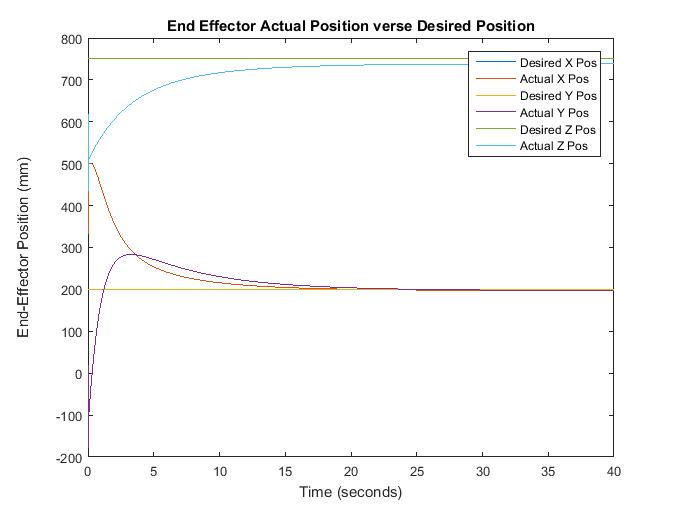
\includegraphics[width=1\linewidth]{matlab_inv_des_act.jpg}
\caption{The desired and actual positions of the end-effector with each joint under control}
\end{figure}
\end{center}

It can be seen in the figure that the error in end-effector position was correctly adjusted, moving the arm from its reset position defined by the D-H parameters to the desired location of $S_d = [200, 200, 750]^T$. Unfortunately, as the control is on two degrees of freedom, and the end-effector's position is in 3 dimensional space, there is uncorrected steady-state error in the z-coordinate.


\begin{center}
\begin{figure}[htb]
  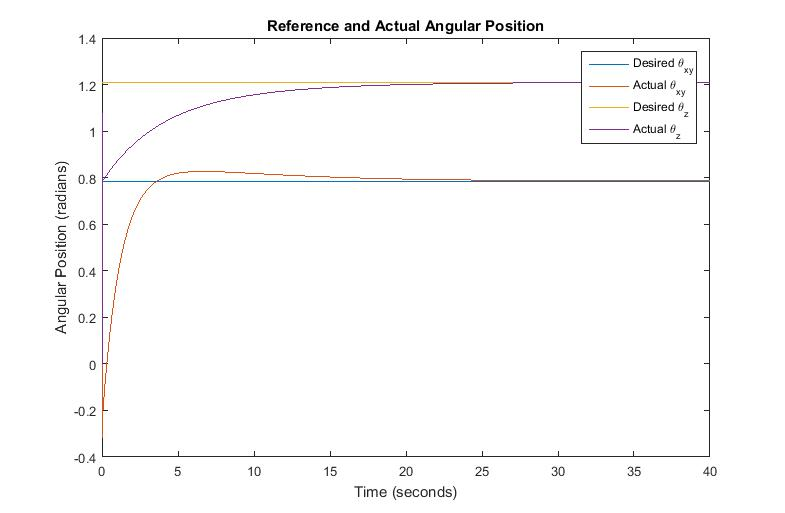
\includegraphics[width=1\linewidth]{matlab_inv_des_act_angle.jpg}
\caption{The desired and actual angular positions of the end-effector}
\end{figure}
\end{center}

It can be seen in the figure above that the desired angular positions were achieved, however, from this prospective there isn't control on radial distance, leading to stead-state error; like there would have been if error in three (angular or linear) displacements were used. Another issue with this controller is that the convergence of $\theta_{xy}$ is faster than $\theta_z$, which is the opposite to that of which is desired, and is a direct consequence of incorrect implementation a reference position correction with integral gain.

\begin{center}
\begin{figure}[htb]
  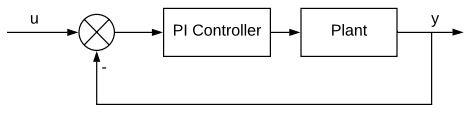
\includegraphics[width=0.8\linewidth]{control_system.jpg}
\caption{Standard Regulator Block Diagram}
\end{figure}
\end{center}

Instead, it would be desirable to use 'integral action', shown below, as it provides a reference position that eliminates steady-state error, and is robust to disturbances.

\begin{center}
\begin{figure}[htb]
  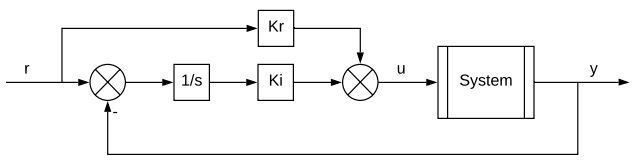
\includegraphics[width=1\linewidth]{control_system_integral_action.jpg}
\caption{Block Diagram of integral action, giving the output (y) a reference input (r)}
\end{figure}
\end{center}


A separate method to achieving the desired response would be to have a cascade loop, regulating $\theta_z$ in the faster inner loop, and $\theta_{xy}$ in the outer-loop, as presented below.

\begin{center}
\begin{figure}[htb]
  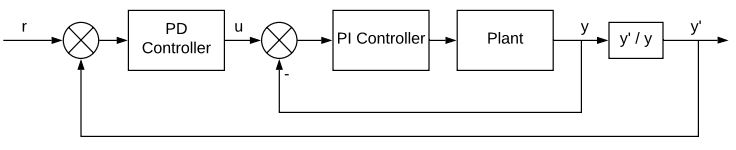
\includegraphics[width=1\linewidth]{control_system_cascade.jpg}
\caption{Block Diagram of a Standard Cascade Regulator}
\end{figure}
\end{center}

The proposed control system was incorporated into the V-REP client program, and the parameters further tuned by exporting the position of the end-effector to a spread sheet, which allowed plotting of the responses. Provided below is a graph showing the error of the controller that was designed within the client program, where an increase in radial distance of the end-effector by 3 mm was desired. It can be seen that steady-state error occurs in $\theta_z$, as found in the simulation, however $\theta_{xy}$ reaches and stays at exactly 0.

\begin{center}
\begin{figure}[htb]
  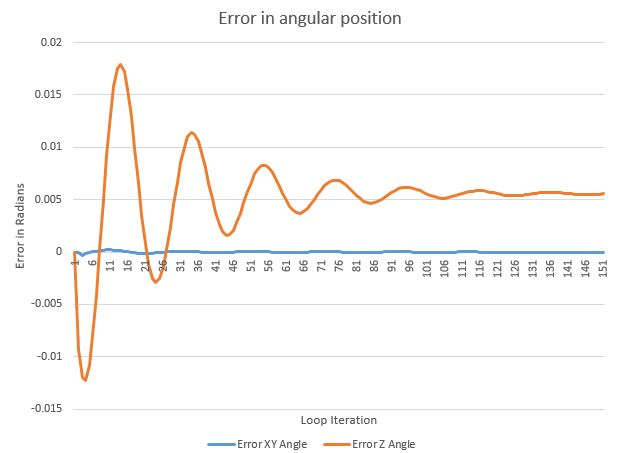
\includegraphics[width=1\linewidth]{control_loop_error.jpg}
\caption{V-REP Client Program Control Loop Error}
\end{figure}
\end{center}


The table below presents the chosen controller gains, and the percentage of error in angle contributed to the total error seen by each controller.

\begin{center}
\begin{table}[htb]


    \begin{tabular}{| p{1.2cm} | p{2cm} | p{2cm} | p{2cm} | p{2cm} | p{2cm} | p{2cm} |}
    \hline
    Joint & $K_p$ & $K_I$ & \% XY & \% Z & Arm Length & Angle Correction \\ \hline
     1 & 0.05	& 0.99	& 100	& 0		& 197.13 &	-$q_1 - \pi$ \\ \hline
     2 & 0.65	& 0.55	& 25	& 75	& 410 	&	$q_2 - \frac{\pi}{2}$  \\ \hline
     3 & 1.17	& 1.11	& 25	& 75	& 207.3 &	$q_3 + \frac{3 \pi}{2}$ \\ \hline
     4 & 0.1	& 0.02	& 50	& 50	& 74.1	& $q_4$ \\ \hline
     5 & 0.15	& 0.15	& 50	& 50 	& 74.1	& $q_5 - \pi$ \\ \hline
     6 & 0.15	& 0.15	& 0		& 0 	& 160 	& $q_6$ \\ \hline
    \end{tabular}
    \caption{Chosen controller coefficients for each joint}
\end{table}
\end{center}


\section{Inverse by Jacobian}
Within this theory section of this report is was found that the Jacobian can be found from the transformation matrix for a robotic manipulator. Following the creation of the transformation matrix for the Kinova Jaco arm, the Jacobian was approach was trialled; in the MATLAB file 'jacobianInverseKinematics.m'.

The first step was to retrieve the expressions that describe the change in linear and rotational positions of the end-effector due to a change in each angle. 

\begin{enumerate}
  \item Firstly, the rotational and translational matrices were extracted from the transformation matrix
  \item The components of the Jacobian representing the change in translational coordinates was filled by deriving the three position states by each joint angle
  \item From this, the rotational matrix can be derived with respect to each angle, creating $\frac{\delta R}{\delta q_i}$
  \item The Skew matrix was created, by $S(\omega) = \frac{\delta R}{\delta q_i} \times R^T$
  \item $\omega_x$, $\omega_y$ and $\omega_z$ were extracted from the skew matrix; representing the change in rotation of the end-effector due to a change in angle $q_i$ 
  \item The rotational components were added to the required position within the Jacobian matrix.
  \item With the Jacobian matrix complete and in symbolic form, substitution of angles of the Jaco arm in a known, not singular, position was substituted into the Jacobian.
  \item The Jacobian could now be inverted; note that the symbolic representation of the Jacobian is overly complex, a symbolic representation of the inverse Jacobian could not be computed.
  \item Substituting these same angles into the transformation matrix leads to the end-effector location in this configuration known.
  \item A vector representing $\frac{dX}{dt}$ needed to be created, the arbitary position $[0, 0, 3, 0, 0, 0]^T$ was used, representing only a change in height by 3 mm; it was found that small changes in position lower than 1 took more iterations to get an accurate approximation.
  \item The change in angles were calculated $\frac{dq}{dt} = J^{-1} \frac{dX}{dt}$.
  \item This change in angle should be multiplied by the change in time (0.025 was used); in a sense this is a proportional gain that restricts over-shooting the desired end-effector position by incrementing in too large of angles. Thus the change in angle is known to be: $\Delta q = \Delta t J^{-1} \frac{dX}{dt}$
  \item The approximated angles for the desired end-effector position could be calculated by $q_{k+1} = q_k + \Delta q$
  \item Substituting $q_{k+1}$ into the transformation matrix could provide the new location of the end-effector.
  \item Re-calculation of the desired change in position, $\frac{dX}{dt}$,  is required to narrow down on an accurate approximation of $\vec{q}$ as per the Newton-Raphson Method; $\frac{dX}{dt}$ = starting position + desired change in position - new calculated position of the end-effector.
  \item Steps 7 to 15 were repeated 50 times to narrow down on an accurate approximation of joint angles for the desired end-effector position.
\end{enumerate}

The results of this process is illustrated in the figure below, where it can be seen that the z-coordinate of the end-effector converges towards the desired position. It can also be noted that as the error in the x and y positions starts to diverge, the method begins to return it to the desired locations. Considering the displacements are in millimeters, this approximation of the end-effector position is usefully accurate for this thesis.


\begin{center}
\begin{figure}[htb]
  \includegraphics[width=1\linewidth]{jacobian_plot.jpg}
\caption{Plot of using Jacobian Approximation to move the end-effector to a desired position }
\end{figure}
\end{center}

Unfortunately however, as aforementioned, the symbolic representation of the Jacobian calculated for this robotic arm is lengthy and consists of harsh trigonometric expressions. A very small sample of the sixth row, first column of the Jacobian is provided below; which can be seen to have conjugates of angles.

$\left(1.0\, \cos\!\left(\overline{\mathrm{q6}}\right)\, \left(0.75\, \sin\!\left(\overline{\mathrm{q4}}\right)\, \left(\cos\!\left(\overline{\mathrm{q1}}\right)\, \cos\!\left(\overline{\mathrm{q2}}\right)\, \cos\!\left(\overline{\mathrm{q3}}\right) + \cos\!\left(\overline{\mathrm{q1}}\right)\, \right),\right)\right)$
 
Unfortunately these expressions cannot be written in C; unless code for conjugate is written. Thus, this Jacobian matrix cannot be easily integrated into the client program. To simplify the Jacobian, the rotational states of the end-effector were excluded from the matrix, reducing the amount of constraints forming the solution. This leads to the Jacobian being rank deficient, which can be overcome with the use of the Pseudo-Inverse Jacobian method; outlined in theory. This method forms a square matrix of size 6, which describes an under-actuated robotic arm. The same process as outlined above was used, again, before inverting the symbolic variables were substituted with the joint positions. It was found that this method did not require step 16, as in the approximation did not require re-iteration to provide a better result, as the end-effector position was within the required accuracy. This significantly reduced the computation time of the solution, and the symbolic Pseudo Jacobian was less complicated than that previously found.

For a change in position $\Delta X = [0, 0, 3, 0, 0, 0]^T$, from an end-effector position of $S_a = [344.4863, 219.7989, 488.1665]^T$, the calculated position was found to be $S_{calc} = [ 344.4755, 219.79189, 491.1696]^T$. The change in angles for this new end-effector position was $\Delta q = [0.0001232, -0.0024076, -0.00240756, 0.000061, 0.00020, 0]^T$. Therefore, it was found that this provided an adequate solution to the inverse kinematics problem, that could be recreated in the client program; MATLAB can convert expressions to C code given they are simple enough. From this, the symbolic representation of $J J^T$ was copied into the client program as a 2-D array of doubles. 

When the client program is working with a forward kinematics scene, it moves the Jaco arm into a configuration without singularities;

\begin{center}
\begin{figure}[htb]
  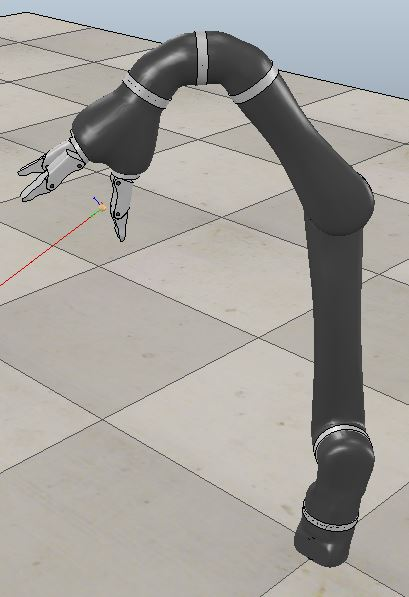
\includegraphics[width=0.5\linewidth]{jaco_start_config.jpg}
\caption{ Starting position of the Jaco arm when giving IK inputs to a FK scene }
\end{figure}
\end{center}

This configuration corresponds to the angles, referenced to the D-H configuration, of

$q = [-8.6394, 1.74581, 10.47175, 4.71239, 0.000001, \pi]^T$

Substituting these angles into the matrix elements gives a result equivalent to that from MATLAB for $J J^T$.


$J J^T = $
$ \left(\begin{array}{ccccc} 
1.4889e5 & -3.81914e3 & -1.3779e2 & -9.6326e4 & 6.77427e4 \\ 
-3.81615e3 & 3.0065e5 & -1.15784e5 & 4.24957e-1 & 3.113135e-1 \\ 
-1.37792e2 & -1.15784e5 & 9.901883e4 & -1.488897e-1 & -7.42055e-2 \\ -9.6325e4 & 4.24857e-1 & -1.488897e-1 & 6.235711e4 & 4.3853e4 \\
-6.77426e4 & 3.11313e-1 & -7.42055e-2 & 4.38533e4 & 3.08403e4 

\end{array}\right)
$

%http://www.ccodechamp.com/c-program-to-find-inverse-of-matrix/
As per the theory, the next step is to inverse $J J^T$, and then multiply this by J, resulting in $J (J J^T)^{-1}$. The inverse of this matrix is computed by calculating the matrix of minors, matrix cofactors, adjugate, and then dividing through by $1/det(JJ^T)$; the general process for calculating the inverse of a nxn matrix in C. Before starting this, the determinant of $J J^T$ is calculated to ensure the matrix is invertible.

In the V-REP client program, the determinant is calculated to be -1.723682e-29 for the starting configuration of the arm. For this same position, MATLAB calculates the determinant to be -6.90106775e-43, thus the calculations are off by a power of -13 before the inverse is calculated. As the determinant is not equal to 0, the inverse was calculated, resulting in a matrix with coefficients magnitudes different to that computed in MATLAB for the same angles. Occasionally, the determinant is calculated in the client program to be $-inf$ despite the arm not being moved. This leads to the belief that the smallest of variances in angles can lead to incorrect results; a direct result of the precision in calculations between MATLAB and C. In the client program, the code has been written for this implementation, but was found to be unsuccessful when it came to computing the inverse of the Pseudo Jacobian, and thus was unable to be used; the client program can enter the functions for these calculations, and display the results, when receiving IK inputs and 'Mode 3' is active.


\chapter{Results Summary and Discussion}
\section{Jaco Arm Control}
The Jaco arm was successfully loaded into the V-REP scene, and was able to be set to both inverse and forward kinematics modes. In the inverse kinematics mode, it was found that control over all six position states was enabled; the tip object could be set to mimic the target object in both translational and rotational position. The focus was to create a means of moving the end-effector from one set of coordinates to another, which was implemented by changing the target's translational position; with the only restriction on angle being that the gripper pointed in the same direction as the target is in the x-y plane. No means of changing the orientation of the end-effector by providing an input was integrated into the client program, however there is a function within the client program designed to vary orientation of objects within V-REP. It may be beneficial to set the joystick up to swap between position control and orientation control, such that the joysticks can either toggle a change in position (as current) or toggle a change in target orientation. To switch between modes, a button on the controller could be pressed; already an output from the joystick process.

It was found that there is no way to change joint angles once V-REP identifies a set of links as an inverse kinematics group. By default, the arm is configured in the upright position with singularities occurring at joints 2 and 3, the Pseudo-Inverse kinematics method for moving the end-effector to the target position could not be used. V-REP's Damped Least Squares inverse kinematics solver however was able to correctly move the Jaco arm despite this, and within 5 iterations always stably moved the end-effector to the target position, in real-time. Using this method with the joystick proved that the Jaco arm was able to be controlled using a joystick seamlessly. 

Once the transformation matrix for the arm was determined, the tip object from the inverse kinematics method was able to be used to indicate the position calculated by the forward kinematics. Thus, it was found that the forward kinematics defines the movement of a point slightly above the last joint of the gripper's 'thumb'. By typing 'fk' as input into the client program, the translational component of the transformation matrix is used to compute the tip position, which is accurate to 0.5 of a millimetre in each coordinate. The transformation matrix in this case is formed using the classic D-H parameters from the Jaco arm documentation, and the translational components were extracted from MATLAB, however there is a separate set of D-H parameters included in the client program which are used to calculate the transformation matrix. With the former method producing accurate results, the calculation of the transformation matrix in the client program is not used.

\begin{center}
\begin{figure}[htb]
  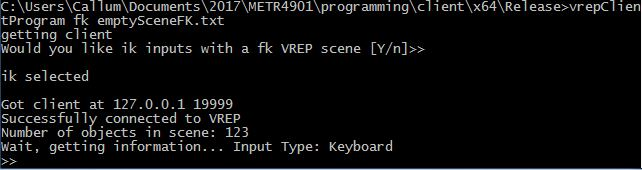
\includegraphics[width=\linewidth]{client_start_up.jpg}
\caption{ Client Program on Start-Up }
\end{figure}
\end{center}
The input arguments of the client program are;

vrepClientProgram.exe fk/ik [object filename] [IP Address] [port]

On start-up, the client will connect to local host on port 19999 unless a IP address and port is specified in the program usage. Once connected, it will prompt for the user to wait while it creates the joystick process and determines if a joystick is connected. When a joystick is connected, it will flag that it found the joystick and is ready for commands, otherwise it will prompt for a keyboard input. The input commands can either be for forwards kinematics for moving a joint angle a given amount of degrees, or inverse kinematics commands that move the end-effector set distances radially from or circularly around the base of the arm. If the user doesn't specify an object filename, it will use the hard-coded object handles for the joints; which may be different if a new scene is created and the Jaco arm isn't the first object to be imported. 
When an input argument to the client specifies that the 'scene' (Jaco arm in V-REP) is in inverse kinematics mode (specified by 'ik'), the target object will be moved and V-REP will calculate the angles to follow. If a scene isn't specified or the input arguments are incorrect, the user will be prompted for each argument individually. When 'fk' is specified as an input argument, the user will be asked whether they desire input arguments of type inverse or forwards kinematics. The separation of these is due to the separation of giving forwards kinematics inputs when the scene is in forwards kinematics mode compared to when the scene in in inverse kinematics mode. Additionally, when the program is set to take inverse kinematics inputs but the scene is in forwards kinematics mode, the Jaco arm needs to be moved into a usable configuration for the inverse methods used; without singularities and with joint 4 of the Jaco arm in the same quadrant as the gripper, with the gripper further out radially.

\begin{center}
\begin{figure}[htb]
  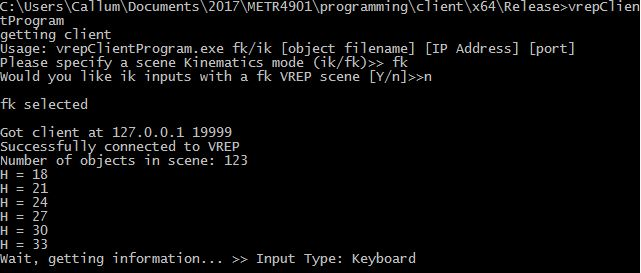
\includegraphics[width=\linewidth]{client_prompted_start_up.jpg}
\caption{ Client Program given incorrect arguments on start-up }
\end{figure}
\end{center}

\section{Joystick Implementation and Processing Time}
Several methods of getting the commands from the joystick were trialled before the SDL solution was found. A comparison of these is found in the appendix, although it is believed that this method provided the best solution as it was a console based application which was easily modifiable in Visual Studio. This program was changed to send only the information necessary for moving the end-effector to the V-REP client program, which communicated through stdin and stdout. It was found that the application wouldn't exit if there wasn't a joystick available. Thus, the application was made to send whether or not there is a joystick to connect to on start up, and exiting if there isn't, allowing the client program to take inputs from keyboard instead of joystick. The joystick application originally used 17\% CPU usage when reading form the joystick. Upon closer inspection, it was found that the program was continuously searching for events on the joystick; it wasn't going to sleep to allow other programs to run more often. MSDN has a function called 'sleep' which will set the thread to wait state, which was used for 50ms within this application. It was found that this figure reduced the CPU usage to below 1\% whilst not taking away from the responsiveness of the application to joystick events.

Upon further inspection of the CPU usage whilst using the V-REP client, it was found that the client program consumed 25\% of the CPU on average. Considering it consisted of one thread for calculations and communication with V-REP, one for reading and interpreting from the joystick process, and one for adding to the buffer when the joystick hasn't been moved and the last log was non-zero, this figure was understandable, however unnecessary. The latter thread hangs in a loop until 750 ms (varies computer to computer depending on CPU speed, but this number was found to be good for the computer this thesis was constructed on) has passed, where it checks the buffer and adds a new command if needed. Thus, it was desirable to make this thread terminate if there isn't a joystick to read from, and when there is, sleep for 50ms to allow other threads to run (meaning a new command is added every 750 - 800 ms, which is an unnoticeable change for the user. A similar outcome was made for the thread that communicates with the joystick process. The main thread was also put into wait state, for 20ms, when it's held waiting for an input command. Overall, it was found that these implementations decreased the CPU usage to around 1\%. It was also evident that the inverse kinematics calculations were performed at around 500 ms (depends on computer CPU), as opposed to the prior average of 750 ms; these results can be seen in the inverse kinematics spread-sheets. Thus, adding waiting delays within the threads allowed the important computations happen quicker, which led to a faster client program.


\section{Client Program Inverse Kinematics}
With setting up the client to be able to interpret inverse kinematics commands, it was found that errors commonly occurred when the end-effector moved between quadrants.  For instance, with the implementation of the proposed analytic inverse kinematics solution (judging the change in end-effector position by moving position of the fourth joint), scenarios occurred where the fourth joint was in one quadrant, and the end-effector in another. This would produce an error when the client program attempts to align the position of the fourth joint with the end-effector, and when it bases calculations for the new end-effector position off a joint which is in a different quadrant. To overcome this problem, when the end-effector is found to be pointing straight upwards, or in a different quadrant to the fourth joint, the client program will move the fourth joint to align them within the same quadrant before starting the inverse kinematics. Errors can still occur when the gripper sits on the negative x-axis, as $q_1 = 0 = 2\pi$, causing undesirable movements to a target angle, or the position of joint 4 could have a small positive y component, and the tip have a negative y component, causing the client program to think the arm is in different quadrants, and get held trying to align something that is visually aligned without flipping the wrist around. As with the physical Jaco arm, it is recommended that this virtual arm only moves within one quadrant (however it can operate fine without coming near the negative x-axis).


In order to demonstrate the implementation of the three inverse-kinematics methods the client program can provide, commands for swapping between the methods was developed. The input syntax for this is, 'mode (mode number) (boolean value)'; for instance, turning mode 1 off would require the command 'mode 1 0'. Typing only the word 'mode' will display the usage for this command, and show the active modes. The mode numbers are as presented in this paper, the first mode is the analytical solution, the second is a control systems method, and the third is for using the Jacobian inverse.


Extracting data from the control loops to a spread-sheet allowed the tuning of the PI controllers. It could be seen that adjusting certain gains would produce effects in steady-state error, oscillation and setting time. In addition to this, it could be seen which commands the solutions struggled with most. For instance, it was found that the control system implementation was accurate in changing the x-y position of the end-effector, however had high oscillation and steady-state error in the z. This was explained to be due to a lack of constraint on the radial position of the end-effector, and due to a high integral gain on $q_1$ which controls the x-y angular position; thus eliminating stead-state error faster than the error in the z-axis is corrected. To overcome these issues, more than two forms of error should be reduced, as the end-effector moves in 3 dimensional space, and a cascade loop should be used so the responses do not fight.


\section{Client Program Jacobian}
%%http://www.cse.hcmut.edu.vn/~hungnq/courses/501120/docthem/Double%20precision%20floating-point%20format%20-%20Wikipedia.pdf
%%https://au.mathworks.com/help/matlab/ref/det.html
%%https://au.mathworks.com/help/matlab/ref/lu.html
%%https://www.codewithc.com/c-program-for-lu-factorization/
%%https://s-mat-pcs.oulu.fi/~mpa/matreng/eem3_4-3.htm
As found in the Kinematics Approach section, the Jacobian inverse kinematics method was unsuccessfully implemented. In the client program, the determinant of $JJ^T$ would equal 0 when using double-precision floating point numbers, and would equal an incorrect value when using standard floats. For double-precision, the spacing, or error in rounding to a representable number, can be found to be $2^{n-52}$, for a number between $2^n$ and $2^{n+1}$, giving a maximum possible error of $2^{-53}$, which rounds to $1.11022e-16$. Thus, the differences in answers is a consequence of rounding between the finite values available with floating point numbers, and thus is also dependent on the order of arithmetic. An example of this error is shown in the calculations below;

$e = 1 - 3*(4/3 - 1)$

results in
 
$e =  2.2204e-16$

which is evidently twice 1.11022e-16, and is not equal to 0 as it is supposed to. For the computation of the determinant, MATLAB uses the product of diagonals of the matrices from the LU decomposition; where the LU decomposition matrices are calculated by Gaussian elimination. In the documentation for MATLAB's lu function (calculates the lower and upper triangle matrices such that A = L $\times$ U), it is noted that factorisation is a key step in obtaining the determinant, for reasons described above. Both, an LU decomposition method and a standard algebraic way of solving smaller determinants within the matrix, were implemented into the client program to solve for the determinant, with results either approaching -$inf$ or 0. Even when comparing the LU matrices from the client, they are different to that from MATLAB, leading to the conclusion that MATLAB's implementation is structured to minimise the error in calculations, which is lacking in the client program.


\section{Kinova SDK}
Development with the Kinova SDK was not trialled as the initialisation functions require connection to the physical Jaco arm, and thus no testing could be conducted. There are plenty of examples within the SDK that show how to code for moving to a new end-effector position, or changing the target positions for the joint angles. From the examples, it is evident that the program designed to use the SDK and control the physical arm would be hardly dissimilar to the developed client program. It would be required to take in a joint number and a desired angle, where internally it sends the commands to the Jaco arm to work with. As the client program now uses significantly less CPU, and can control the virtual arm in real-time, it is evident that processing to the development of the physical arm's interface can begin.


\section{Data Streaming Implementation}
To be able to detect collisions, the client program comes with a synchronous mode, where it continuously retrieves the Jaco arm's angles from V-REP. In order to do this, 6 threads were created, one for each joint; as only one value can be streamed constantly. Thus, 6 connections are made to V-REP over 6 ports, with the data being streamed every 50 ms (variable). Once a new joint angle arrives to one of the clients, it updates the struct containing the arm parameters, which is accessible by all threads; mutexes make this thread safe, the main thread will only look at the angles when making movement calculations. This mode was deactivated for general use of the client program, as it was found to significantly reduced simulation time (due to V-REP's increased background processing). Another finding was that the simulation time depended on the amount of objects in the scene, as well as the CPU's capabilities; moving to a different computer, it was found that moving the Jaco arm was 5 times faster. Thus, there is potential that the streaming method can work with the client program operating as normal, given an empty scene and a good CPU. To reduce the load on the CPU, the threads sleep for 10 ms whenever data has not arrived from V-REP. This was found to again to decrease processing time, however not enough to implement velocity / acceleration checking; but may be a good option on a better computer. 


%This may be one chapter or several.  Again, titles should be more
%informative than the above.
%
%You will almost certainly need diagrams to clarify your meaning.  The
%\LaTeXe\ \texttt{graphics} package allows the inclusion of PostScript
%graphics, as in \fig{flr1}.  The inclusion of \LaTeX\ \texttt{picture}
%graphics, as in \fig{fzsys}, requires no auxiliary packages and allows
%the mathematical formatting features of \LaTeX\ to be used in
%diagrams; but the \texttt{picture} files, unlike PostScript files,
%usually require manual editing.

%\chapter{Results and discussion \ldots}
%
%\ldots\ or perhaps the discussion should be a separate chapter.
%
%In any case, you will probably need to include tabulated results.
%\tab{tf2} illustrates the use of various \LaTeX\ environments to
%include a computer printout (plain text file) in a document.  The
%\texttt{verbatim} environment, which encloses the formatted text, is
%also useful for program listings.
%
%\begin{table}\renewcommand{\baselinestretch}{1.0}
%\caption{\sl Fraction of air volume involved in heat exchange for
%second mode (right column) vs.\ filling factor (left column).  The
%plain-text headings represent $f$, $m$, $\mu_2$ and $f_2$.}
%\label{tf2}
%
%\begin{center}
%\begin{minipage}[c]{2.85in}\small\normalsize
%\begin{verbatim}
%
% f(%)     m         mu2     f2(%)
%
% 0.016   80.00    0.05400   4.874
% 0.031   56.57    0.07732   5.438
% 0.062   40.00    0.11103   6.125
% 0.125   28.28    0.16001   6.970
% 0.250   20.00    0.23175   8.020
% 0.500   14.14    0.33799   9.329
% 1.000   10.00    0.49789  10.967
% 2.000    7.07    0.74444  13.008
% 4.000    5.00    1.13919  15.525
% 8.000    3.54    1.81095  18.568
%
%19.237    2.28    3.61958  23.174
%37.180    1.64    7.28635  27.094
%57.392    1.32   14.63631  29.813
%74.316    1.16   29.35160  31.453
%85.734    1.08   58.79364  32.360
%\end{verbatim}
%\end{minipage}
%\end{center}
%\end{table}

\chapter{Conclusions}
\section{Summary and Conclusions}
The primary objective of this thesis was to create a client program which uses the V-REP remote API to control a virtual Kinova Jaco arm. Upon forming a method for reliable control, different techniques used for calculating the joint angles required to move the end-effector of a 6 joint robotic arm were studied. Experimentally, the validity of three approaches were tested, to determine which was the most robust in accurately controlling the robotic arm. \\

The first approach used relationships between joints to calculate the angles required to move the arm into an approximate position, and then used control loops to reduce the error in end-effector position. This was found to be successful in most arm configurations, where the joint angles were correctly calculated in 500 ms on an old computer, and an average of 100 ms on a modern laptop. Unfortunately this method led to errors when the arm tried to reach points too close to the z-axis, as some components of the arm were in different quadrants to others.\\

A control systems approach was wrongly implemented into the client program, which allowed the calculation of joint angles which produced an undesirable amount of steady-state error in the height of the end-effector from the base. After reviewing the model used in for this approach, it was found that there is a lack of control on the radial position of the arm, which contributed to the steady-state error, along with having a high integral gain on the control of the x-y axis. Alternative models were proposed which would overcome these problems.\\

The Jacobian was also integrated into the client program after providing good results in MATLAB. Due to calculation differences, and numerical precision, the inverse Jacobian for a given set of joint angles was unable to be calculated with accuracy in the client program. The discrepancy between MATLAB and the client program came from the more sophisticated method of calculating the determinant and inverse of a square matrix in MATLAB; which takes into account the order of operations such that the error due to the rounding of (double) floating point numbers is reduced.\\

Despite these draw-backs, the client program successfully acheived crucial design objectives.

\begin{itemize}
	\item An easy to use program was created which allowes the control of the Jaco arm given forward or inverse kinematics commands.
	\item The end-effector position can be controlled with the use of an external joystick (similar to a PS3 controller).
	\item Mathematical solutions to the forward and inverse kinematics of the Jaco arm are integrated into the V-REP client and produce accurate results.
	\item Collision avoidance can be implemented using the data-streaming capabilities of the client program given a fast enough CPU.
	\item Through V-REP's inverse kinematics solver, set to Damped Least Squares, or the analytical solution provided by the client program, the position of the end-effector of the Jaco arm can be controlled in real time.
	\item The client program created has functions within for further development, such as orientation control of the end-effector, detecting collisions, and sending joint information to other programs.
	\item The client program was optimized for CPU usage and computational efficiency. It can also be quickly modified to allow the printing of usage information associated with different areas of the program, and to allow data-streaming.
\end{itemize}


\section{Developed Files}

In total, the client program contains three .c files and .h files. The main file was designed to do calculations and communicate with V-REP; the flow diagram for which is provided with this document. All kinematics calculations were kept in a separate file to communication, and is used for control loop, forward / inverse kinematics, and computing the inverse Jacobian. The final file, with two threads, is dedicated to controlling the commands coming from the joystick; one for getting and interpreting commands and another for servicing the command buffer, which added commands to the buffer when the joystick is held in a non-zero position. When the threads are waiting for an input, from user, joystick or buffer, the threads are set to a waiting state to limit the CPU usage of the program, which was found to decrease computation time, creating a more responsive system between joystick command and V-REP Jaco arm movements.

All kinematics were trialled in MATLAB before implementing into the client program. This relieved the need for the client program to manipulate complex matrix operations for the forward kinematics. Instead, the calculations were made symbolically in MATLAB and copied over for integration; for instance, in calculating the Pseudo Jacobian, 10 complex expressions describing the elements of $JJ^T$ were able to be copied from MATLAB instead of having the client program compute this relationship each time. The MATLAB files are provided with this document, which include forward kinematics, inverse kinematics, Jacobian inverse and Pseudo inverse calculations, and a Simulink model simulating the control system implemented in the client program.


\section{Possible Future Work}
As noted, unsolved problems occurred in the closing of this thesis. It is believed that with time all of which can be fixed, giving a more complete client program for controlling the virtual robotic arm. As it stands, the client program is able to control the virtual arm in both forward kinematics and inverse kinematics modes, using V-REP to calculate joint angles or using the proposed analytic solution. However, it is evident from the MATLAB script on the inverse Jacobian, that this method can produce accurate results in approximating the change in joint angles required for a small change in end-effector position. This method can be further implemented in two ways;

\begin{itemize}

	\item Using the symbolic $JJ^T$ matrix in the client program for the Jaco arm, construct a method for computing the determinant and inverse in a similar means to MATLAB, to ensure transparent results across platforms; MATLAB uses LU decomposition solved by Gaussian elimination, whereas the client program uses a simplified version of this which is susceptible to rounding errors.
	\item V-REP has an internal function, simComputeJacobian, which provides the last linearised Jacobian matrix of an inverse kinematics group. This functionality, and more, are available in the External Kinematics Library, which is an auxiliary API not directly a part of V-REP. Example code for using this library is provided with V-REP on download, and is written in C++. With an original lack of knowledge of how these functions work, and what the matrices represent, this avenue was not greatly explored. With more knowledge now, it can be seen to be a useful library to incorporate into the client program.

\end{itemize}

Additionally, it was found that the control system implementation was able to converse two of the three axis of the tip to a desired end-effector position. The steady-state error in the z-axis can be eliminated by making the following design considerations;

\begin{itemize}

	\item Having control over the error in three axis, polar or Cartesian, instead of two; which were the polar angles in the x-y plane and xy-z plane. Reducing the control to two, being the x-y and z angles, reduces the control of the end-effector in 3-Dimensional space.
	\item It was known that $q_1$ would have a large influence on correcting the error in the x-y plane, and the other joints would have a coupling of all three axis. A high integral gain was set to control $q_1$, with the expectation that the other joints would position the end-effector close to the desired position, with any error in the x-y plane being slowly corrected by the control of $q_1$. Instead, the high integral gain created a faster response than the other joints. Reflecting on the model used, this is understandable as integral gain intrinsically increases rise-time and overshoot. Outlined in the Kinematics Approach section is the two models which were supposed to be used to meet the design goals. These are to implement integral action, or similarly a cascade loop, which brings $q_1$ to a reference position with a slow enough response that it does not effect the regulation of the other joint angles.

\end{itemize}

Data-streaming was proven to be successful, however V-REP became slow with communicating with each joint angle to the client continuously. For future improvements of this, it is recommended to try the data-streaming mode of the client program on a computer with a better CPU. Additionally, an internal LUA script can be created to detect collisions using V-REP's collision detection feature, and communicate with a thread in the client program when there is a collision. Thus, this would change the number of threads required for collision detection to 1 instead of 6 plus acceleration calculations; which may result in false positives. It was found that communicating with V-REP with over 7 threads can cause the program to crash, and thus the number of threads connecting to V-REP should be limited.

With these developments, and the current state of the client program, it is believed that the application for controlling the physical Jaco arm can be created.

\appendix

% Chapters after the \appendix command are lettered, not numbered.
% Setting apart the appendices in the table of contents is awkward:

\newpage
\addcontentsline{toc}{part}{Appendices}
\mbox{}
\newpage

% The \mbox{} command between two \newpage commands gives a blank page.
% In the contents, the ``Appendices'' heading is shown as being on this
% blank page, which is the page before the first appendix.  This stops the
% first appendix from be listed ABOVE the word ``Appendices'' in the
% table of contents.

% \include appendix chapters here.

\chapter{Appendix}
\section{Joystick Applications}
\subsection{Objectives}
•	Retrieve real time data of the joystick states; button presses and joystick position from a Generic Joystick Controller with USB input.
•	Have the states printed to stdout in real time using an executable that can be spawned from a parent process (VREP main client).
•	The process must be killable from the parent process as well, to avoid unnecessary hanging and infinite forking, which could damage computer memory.

\subsection{Windows API}
Windows has its own API for building window executables. This API is formatted differently to standard C programs, and contains very different properties and types. For example, main is run from [1]:
int WINAPI WinMain(HINSTANCE hInstance, HINSTANCE hPrevInstance, LPSTR lpCmdLine, int nShowCmd){
The syntax and libraries from Windows.h, with hidsdi.h allowes direct communication with Human Interface Devices (HID). Windows are generated first, and messages are sent through this thread and the HID, thus to GetRawInputData(), a window must be created to generate the message struct [1] and the lParam argument [2]. Message windows can be created by setting the hWndParent parameter of CreateWindow() to HWND\_MESSAGE; this will create a hidden window that can only be terminated using Task Manager. 
The primary problem with the Windows API is that it is separate to the console, thus writing to stdout is ineffective, and the only way to create an output is to write to a file with FILE* f = fopen(), and fprintf(f, “text”). Setting the linking configuration from Windows to Console will cause the program build to be unsuccessful. Despite these problems, Windows API provides the lowest level of talking directly to the HID drivers, and manipulation of USB data from the controller.

Open-source code for generating a window containing a joystick GUI with real-time button presses is available from [4]. Building RawInputJoystickSource/Raw Input.vcxproj in Visual Studio will generate an executable Raw Input.exe in RawInputJoystickSource/Debug, which can be run from command prompt. Adding print statements or writing to stdout won't produce anything on command prompt, however the executable will create a window containing the joystick visualisation. Re-writing the source code from the Windows API was unsuccessful as getting the raw input requires the message struct, generated using a window thread. Created text files however will appear in /Debug.

\subsection{HTML5 Gamepad API}
Code for creating joystick support with browser (HTML5) games is available from [5] with information at [6]. The latter contains instructions for getting a PS4 controller working in Chrome and Firefox. As this isn’t useful for application based programs, it would be a useful alternative for games that are ran using .html.

\subsection{Libusb and xusb.c}
A library used for retrieving information from USB, with an example executable and solution, xusb.c, which demonstrates this for Generic, PS3 and Xbox joysticks [7]. The library functions have documentation available from [7], however, apart from the xusb example there is limited documentation on how to implement these functions or format code. Thus, manipulating the code for the Generic USB Joystick to work with xusb.c, to see the button inputs is difficult. If the file is ran with “xusb.exe –s vid:pid” the device information and reading input report can be generated, if buttons are being pressed the hexadecimal output will reflect this. It is possible to loop the “Reading Input Report” and print to stdout in the same way as current. The inputs will then have to be mapped to buttons, which can create difficulty with interpreting the state of the joysticks. A PS3 controller code did not work (exited with Input/Output error), as the inputs weren’t printed to terminal, but it is expected that the code format for processing the input, to show which buttons were pressed, will be similar to that for the Generic USB controller. The code can be executed from libusb-1.0.21/examples/bin64, with code kept in libusb-1.0.21/examples/xusb.c.

\subsection{Simple Direct Layer (SDL) Source Code}
Written in C, a cross platform library can be download for the use of getting data from keyboard, mouse and joysticks, from the SDL website [9]. If the source code is modified it must be marked as so, otherwise it is free to be used and manipulated to repeatedly display input data from devices; originally set to only print device information, however input manipulation functions are provided. The joystick project can be built by loading SDL2-2.0.7/VisualC/SDL into Visual Studio and building from testjoystick.c. This file initialises the joystick and retrieves data from the SDL\_joystick.c file, where it can be executed in a console from SDL2-2.0.7/VisualC/Win32/Debug. The test files are setup to produce a GUI, however the code for this can be commented out, and input manipulation moved to main. Printf can be included by creating a new stream pointing to standard out, and joystick information sent to it (by default, SDL uses a different handler (not stdout) to point information to the command line, and so an external process cannot read this information).


\section{Alternate Inverse Kinematics Solutions}

%%%%%%%% Need to move this chunk of text to the appendix...
%https://books.google.com.au/books?id=PK_N9aFZ3ccC&printsec=frontcover&dq=tsai+and+morgan+robotics+textbook&hl=en&sa=X&ved=0ahUKEwjRvqqIw63bAhXGwLwKHRxbDAoQ6wEIUjAH#v=onepage&q&f=false
%https://reader.elsevier.com/reader/sd/B3D6C34BEA5F22FD156A30862B225645F137D5CBAEF54030ADE786D00811AE281D632E6381AF7B9758568981C0ABC1B4
Manipulators with 6 rotational joints can reach any position within its stretched length, where motors with more joints are termed as over-actuated robotic actuators and are capable of changing their joint configurations without changing the end-effector position. It is the aforementioned reason that 6 joint robotic arms are of such large interest, and the inverse kinematics is of such high interest.\\
Raghavan and Roth's solution to the inverse kinematics of any 6 joint robotic arm is identified in many research papers and textbooks. It takes the transformations matrices from the forward kinematics, and rearranges them to make a system of equations about joint three. From here, there are 6 unknowns and 5 equations, where by substituting out the trigonometric products form a linear system with 16 unknowns and 6 equations. With more substitutions they arrived at a 12 by 12 matrix written in terms of variables representing trigonometric expressions. The determinant of this matrix gives a 16-degree polynomial referenced to the middle joint, of which can be solved for using a root solver, and the other joint angles found by back substitution. From this, it was concluded that there is 16 possible solutions to the inverse kinematics, however solving a 16-degree polynomial made this method too slow for real-time implementation. The Manocha Method avoids solving the determinant by forming the equations into an eigenvalue problem, where in solving for the eigenvectors gave three of the arm's joint angles with less operations. This was the first real-time inverse kinematics method to be implemented, with methods since being variations of the two outlined above. The Raghavan and Roth method is briefly outlined in appendix C of Lung-Wen Tsai's textbook Robot Analysis: The Mechanics of Serial and Parallel Manipulators. Further, it is worked through along with the Manocha Method in an article from the 14th Triennial World Congress, 1999, A Faster Algorithm for Calculating the Inverse Kinematics of General 6R Manipulator for Robot Real Time Control.\\
It is believed that although new methods derived from those described above form solutions to the inverse kinematics problem in this thesis, as the Jaco arm has 6 revolute joints, the mathematics knowledge and tools for computing the eigenvalues of the complex equations is insufficient.\\

\section{Appendices notes}
Appendices are useful for supplying necessary details or explanations
which do not seem to fit into the main text, perhaps because they are
too long and would distract the reader from the central argument.
Appendices are also used for program listings.

Notice that appendices are ``numbered'' with capital letters, not
numerals.  When the \verb+\appendix+ command in
\LaTeX~\cite[p.\,175]{lamport} is used with the \texttt{book} document
class, it causes subsequent chapters to be treated as appendices.

\chapter{Program listings}

\section{First program}

Some initial explanatory notes may precede the listing.

\section{Second program}

\section{Etc.}

\chapter{Companion disk}

If you wish to make some computer files available to your examiners,
you can list and describe the files here.  The files can be supplied
on a disk and inserted in a pocket fixed to the inside back cover.

The disk will not be needed if you can specify a URL from which the
files can be downloaded.

\cleardoublepage

\begin{thebibliography}{99}
\addcontentsline{toc}{chapter}{Bibliography}
\bibitem{lamport} L.~Lamport, \emph{\LaTeX: A Document Preparation
System}, 2nd ed. (Addison-Wesley, 1994).
\bibitem{LABEL2} REFERENCE 2
\bibitem{ETC.} Etc.
\end{thebibliography}

\end{document}